% ==========================================================================
%  Guia de Estudo — Prova 1 / Lista I
%  Macroeconomia I (PPGEco-UFES, 2026)
%  Prof. Ricardo Ramalhete Moreira
%  Baseado nos padrões da P1 2024 e na Lista I 2026
% ==========================================================================
\documentclass[12pt, a4paper]{article}

% --------------------------------------------------------------------------
% Packages
% --------------------------------------------------------------------------
\usepackage[utf8]{inputenc}
\usepackage[T1]{fontenc}
\usepackage[brazil]{babel}
\usepackage{lmodern}
\usepackage{microtype}

\usepackage[top=2.5cm, bottom=2.5cm, left=3cm, right=3cm, headheight=15pt]{geometry}

\usepackage{amsmath, amssymb, amsthm}
\usepackage{mathtools}
\usepackage{bm}

\usepackage{graphicx}
\graphicspath{{lista_I/figures/}{figures/}}
\usepackage{float}
\usepackage[font=small, labelfont=bf, justification=justified]{caption}
\usepackage{subcaption}

\usepackage{booktabs}
\usepackage{array}
\usepackage{multicol}
\usepackage{xcolor}
\usepackage{hyperref}
\usepackage{enumitem}
\usepackage{tcolorbox}
\tcbuselibrary{breakable}

% --------------------------------------------------------------------------
% Cores
% --------------------------------------------------------------------------
\definecolor{cyanrbc}{HTML}{3b9dbd}
\definecolor{orangerbc}{HTML}{d97b39}
\definecolor{grayrbc}{HTML}{6b7280}
\definecolor{greenbox}{HTML}{166534}
\definecolor{greenbg}{HTML}{dcfce7}
\definecolor{boxbg}{HTML}{f5f0e8}
\definecolor{boxborder}{HTML}{3b9dbd}
\definecolor{provabg}{HTML}{fff7ed}
\definecolor{provaborder}{HTML}{d97b39}

% --------------------------------------------------------------------------
% Caixas (standard skin — sem skins/TikZ para evitar manchas negras)
% --------------------------------------------------------------------------
\newtcolorbox{resultbox}[1][]{standard, colback=boxbg, colframe=boxborder,
  boxrule=1pt, arc=3pt, left=6pt, right=6pt, top=4pt, bottom=4pt,
  fonttitle=\bfseries\small, #1}
\newtcolorbox{provabox}[1][]{standard, colback=provabg, colframe=provaborder,
  boxrule=1.2pt, arc=3pt, left=6pt, right=6pt, top=4pt, bottom=4pt,
  fonttitle=\bfseries\small, #1}
\newtcolorbox{formulabox}[1][]{standard, colback=greenbg!30, colframe=greenbox!60,
  boxrule=0.8pt, arc=3pt, left=6pt, right=6pt, top=4pt, bottom=4pt,
  fonttitle=\bfseries\small, #1}

% --------------------------------------------------------------------------
% Comandos matemáticos
% --------------------------------------------------------------------------
\newcommand{\E}{\mathbb{E}}
\newcommand{\dif}{\mathrm{d}}
\newcommand{\khat}{\hat{k}}
\newcommand{\chat}{\hat{c}}
\newcommand{\yhat}{\hat{y}}
\newcommand{\zhat}{\hat{z}}
\newcommand{\rstar}{r^*}
\newcommand{\kstar}{k^*}
\newcommand{\cstar}{c^*}

% --------------------------------------------------------------------------
% Espaçamento e parágrafos
% --------------------------------------------------------------------------
\setlength{\parskip}{0.5\baselineskip}
\setlength{\parindent}{0pt}

% --------------------------------------------------------------------------
% Títulos
% --------------------------------------------------------------------------
\usepackage{titlesec}
\titleformat{\section}{\large\bfseries\color{cyanrbc}}{Questão \thesection.}{0.5em}{}[\vspace{-0.3em}\rule{\linewidth}{0.4pt}]
\titleformat{\subsection}{\normalsize\bfseries\color{grayrbc}}{}{0em}{}

% --------------------------------------------------------------------------
% Cabeçalho/rodapé
% --------------------------------------------------------------------------
\usepackage{fancyhdr}
\pagestyle{fancy}
\fancyhf{}
\lhead{\footnotesize\textcolor{grayrbc}{Guia P1 --- Macroeconomia I (PPGEco-UFES, 2026)}}
\rhead{\footnotesize\textcolor{grayrbc}{RCK \& RBC --- Romer, cap.\ 2--5}}
\cfoot{\small\thepage}
\renewcommand{\headrulewidth}{0.4pt}

% ==========================================================================
\begin{document}
% ==========================================================================

% --------------------------------------------------------------------------
% Capa
% --------------------------------------------------------------------------
\begin{titlepage}
\begin{center}
\vspace*{1.5cm}
{\Large\bfseries Universidade Federal do Espírito Santo}\\[0.5em]
{\large Programa de Pós-Graduação em Economia (PPGEco-UFES)}\\[2em]

\rule{\linewidth}{1.2pt}\\[0.8em]
{\LARGE\bfseries\color{cyanrbc} Guia de Estudo --- Prova 1 / Lista I\\[0.4em]
\large Macroeconomia I --- 2026}\\[0.8em]
\rule{\linewidth}{1.2pt}

\vspace{1em}
{\large Prof.\ Ricardo Ramalhete Moreira}

\vspace{1.5em}
\begin{tcolorbox}[standard, colback=provabg, colframe=provaborder, width=0.88\textwidth,
  arc=4pt, boxrule=1.2pt, left=8pt, right=8pt, top=6pt, bottom=6pt]
\centering
\textbf{\textcolor{provaborder}{Atenção:}} Este guia foi elaborado com base no
padrão da \textbf{P1 2024} e nas questões da \textbf{Lista I 2026}.\\[0.3em]
Cobre os modelos \textbf{RCK} (Romer, cap.\ 2) e \textbf{RBC} (Romer, cap.\ 5),
que constituem o conteúdo de prova 1.
\end{tcolorbox}

\vspace{1.5em}
\begin{tabular}{ll}
\textbf{Questões 1--3:} & Modelo de Ramsey-Cass-Koopmans (RCK) \\[0.4em]
\textbf{Questões 4--8:} & Modelo de Ciclos Reais de Negócios (RBC) \\[0.4em]
\textbf{Apêndice:} & Questões-tipo P1 (estilo 2024)
\end{tabular}

\vspace{1.5em}
\begin{tcolorbox}[standard, colback=boxbg, colframe=boxborder, width=0.88\textwidth,
  arc=4pt, boxrule=1pt, left=8pt, right=8pt, top=6pt, bottom=6pt]
\centering
\textbf{Referência principal:} \\[0.3em]
D.\ Romer, \textit{Advanced Macroeconomics}, 5.ª ed., McGraw-Hill (2019). \\
Capítulos 2 e 5.
\end{tcolorbox}

\vfill
{\small Soluções computadas com Python; código disponível em
\texttt{github.com/fcarva/macro}.}
\end{center}
\end{titlepage}

% --------------------------------------------------------------------------
% Formulário de Referência Rápida (pág. 2)
% --------------------------------------------------------------------------
\newpage
\thispagestyle{fancy}

\begin{center}
{\large\bfseries\color{cyanrbc} Formulário de Referência Rápida --- P1}\\[0.3em]
\rule{\linewidth}{0.6pt}
\end{center}

\vspace{0.3em}
\begin{multicols}{2}

\textbf{\textcolor{cyanrbc}{BLOCO RCK}}

\medskip
\textbf{Utilidade CRRA:}
\[
u(c) = \frac{c^{1-\theta}-1}{1-\theta}, \quad u(c)=\ln c \;\text{(}\theta=1\text{)}
\]

\textbf{Keynes-Ramsey (consumo per-cápita):}
\[
\frac{\dot{c}}{c} = \frac{r - \rho}{\theta}, \quad r = f'(k)-\delta
\]

\textbf{Keynes-Ramsey (unidade efetiva):}
\[
\frac{\dot{\tilde{c}}}{\tilde{c}} = \frac{f'(\tilde{k}) - \delta - \rho - \theta g}{\theta}
\]

\textbf{Estado estacionário:}
\[
\rstar = \rho + \theta g, \quad \kstar = \!\left(\frac{\alpha}{\rstar}\right)^{\!1/(1-\alpha)}
\]
\[
\cstar = (\kstar)^\alpha - (\delta+n+g)\kstar
\]

\textbf{Bem-estar:}
\[
W^* = \frac{u(\cstar)}{\rho} = \frac{\ln\cstar}{\rho} \;(\theta{=}1)
\]

\textbf{Condição de convergência/transversalidade:}
\[
\rho - n - (1-\theta)g > 0
\]

\textbf{Diagrama de fases (4 regiões):}

\begin{center}
\begin{tabular}{p{2.8cm}cc}
\toprule
Região & $\dot{c}$ & $\dot{k}$ \\
\midrule
Esq.\ $\dot{c}=0$, acima $\dot{k}=0$ & $>0$ & $<0$ \\
Esq.\ $\dot{c}=0$, abaixo $\dot{k}=0$ & $>0$ & $>0$ \\
Dir.\ $\dot{c}=0$, acima $\dot{k}=0$ & $<0$ & $<0$ \\
Dir.\ $\dot{c}=0$, abaixo $\dot{k}=0$ & $<0$ & $>0$ \\
\bottomrule
\end{tabular}
\end{center}

\columnbreak

\textbf{\textcolor{cyanrbc}{BLOCO RBC}}

\medskip
\textbf{Estado estacionário do capital:}
\[
I^* = \delta K^*, \quad \beta(\rstar + 1 - \delta) = 1
\]

\textbf{Lei de movimento log-linearizada:}
\[
\khat_{t+1} = A\,\khat_t + B\,\zhat_t, \quad |A| < 1
\]

\textbf{Utilidade com lazer:}
\[
u(C,l) = \ln C + b\ln l, \quad l = 1-N
\]

\textbf{Desutilidade marginal do trabalho:}
\[
\text{DML} = \frac{b}{l} = \frac{b}{1-N}
\]

\textbf{Lazer ótimo (ótimo intratemporal):}
\[
l^* = \frac{bC}{w}, \quad \frac{C}{l} = \frac{w}{b}
\]

\textbf{Substituição intertemporal de trabalho:}
\[
\frac{1-l_1}{1-l_2} = \beta(1+r)\frac{w_2}{w_1}
\]

\textbf{Calibração de $b$:}
\[
b = \frac{w^* l^*}{C^*} = \frac{w^*(1-N^*)}{C^*}
\]

\textbf{3 canais de choque de PTF:}
\begin{enumerate}[leftmargin=1.2em, topsep=0pt, itemsep=1pt, parsep=0pt]
\item Direto: $z\uparrow \Rightarrow Y\uparrow$
\item Invest.: $\hat{I}_0 > \hat{Y}_0$ (amplificação)
\item Suavização: $\hat{C}_0 < \hat{Y}_0$
\end{enumerate}

\medskip
\textbf{Calibração padrão:}\\[2pt]
$\alpha=0.33$, $\beta=0.99$, $\delta=0.025$,\\
$\rho_z=0.95$, $\sigma_z=0.007$, $b\approx 1.55$

\end{multicols}

\rule{\linewidth}{0.6pt}

\vspace{0.5em}
\begin{provabox}[title={Convergência e transversalidade (fórmula mais cobrada)}]
A condição $\rho - n - (1-\theta)g > 0$ garante que a integral de bem-estar converge
\textbf{e} que a condição de transversalidade $\lim_{t\to\infty} k(t)\mu(t)e^{-(\rho-n)t}=0$
é satisfeita. Sem ela, a economia não tem um plano ótimo bem definido.
Na P1 2024, a alternativa incorreta dizia $\rho - n + (1-\theta)g > 0$ --- sinal trocado!
\end{provabox}

% --------------------------------------------------------------------------
% Sumário
% --------------------------------------------------------------------------
\newpage
\tableofcontents
\newpage

% ==========================================================================
%  PARTE I — MODELO RCK (Questões 1-3)
% ==========================================================================

\section*{\large\color{cyanrbc} Parte I --- Modelo de Ramsey-Cass-Koopmans (Q1--Q3)}
\addcontentsline{toc}{section}{Parte I --- Modelo RCK (Q1--Q3)}

O modelo RCK (Romer, cap.\ 2) descreve uma economia de tempo contínuo em que famílias
representativas maximizam o bem-estar intertemporal sujeitas à acumulação de capital.
A solução ótima satisfaz a equação de Ramsey (\textit{Keynes-Ramsey rule}) e a condição
de transversalidade.

\bigskip

% ==========================================================================
\setcounter{section}{0}
\section{Bem-estar no estado estacionário e estática comparativa}

\subsection*{Enunciado resumido}
Encontre $W^* = \int_0^\infty u(c^*)\,e^{-\rho t}\,\dif t$ e analise como
$\theta$, $\rho$, $n$ e $g$ afetam $\kstar$, $\cstar$ e $W^*$.

% ------------------------------------------------------------------
\subsection*{1.1 \ Utilidade instantânea e bem-estar no estado estacionário}

A utilidade instantânea com parâmetro de aversão relativa ao risco $\theta > 0$:
\begin{equation}
u(c) = \frac{c^{1-\theta} - 1}{1-\theta} \qquad (\theta \neq 1),
\label{eq:crra}
\end{equation}
com $u(c) = \ln c$ para $\theta = 1$.

No estado estacionário $c(t) = \cstar$ para todo $t$:
\begin{equation}
W^* = \int_0^\infty u(\cstar)\,e^{-\rho t}\,\dif t = \frac{u(\cstar)}{\rho},
\label{eq:welfare_ss}
\end{equation}
válido se $\rho > 0$.

% ------------------------------------------------------------------
\subsection*{1.2 \ Estado estacionário}

As condições $\dot{k}=0$ e $\dot{c}=0$ implicam:
\begin{align}
f'(\kstar) &= \rstar = \rho + \theta g, \label{eq:rstar}\\
f(\kstar) - \delta \kstar - (n+g)\kstar &= \cstar. \label{eq:cstar}
\end{align}
Com $f(k)=k^\alpha$:
\[
\kstar = \left(\frac{\alpha}{\rstar}\right)^{1/(1-\alpha)}, \qquad
\cstar = (\kstar)^\alpha - (\delta+n+g)\kstar.
\]

% ------------------------------------------------------------------
\subsection*{1.3 \ Estática comparativa}

\begin{table}[H]
\centering
\small
\setlength{\tabcolsep}{5pt}
\renewcommand{\arraystretch}{1.45}
\caption{Efeitos de aumentos paramétricos no estado estacionário do modelo RCK.}
\label{tab:welfare_cs}
\begin{tabular}{@{}lcccc p{6.8cm}@{}}
\toprule
\textbf{Parâmetro} & $\boldsymbol{r^*}$ & $\boldsymbol{k^*}$ & $\boldsymbol{c^*}$ & $\boldsymbol{W^*}$
  & \textbf{Canal de transmissão} \\
\midrule
$\uparrow\theta$
  & \textcolor{blue!70!black}{$\uparrow$}
  & \textcolor{red!70!black}{$\downarrow$}
  & \textcolor{red!70!black}{$\downarrow$}
  & \textcolor{red!70!black}{$\downarrow$}
  & $\theta\!\uparrow\;\Rightarrow\;
     \underbrace{r^*{=}\rho{+}\theta g}_{\text{custo efetivo}}\!\uparrow\;
     \Rightarrow\; f'(k^*)\uparrow\;
     \Rightarrow\; k^*\downarrow\;
     \Rightarrow\; c^*\downarrow\;
     \Rightarrow\; W^*\downarrow$ \\[2pt]
$\uparrow\rho$
  & \textcolor{blue!70!black}{$\uparrow$}
  & \textcolor{red!70!black}{$\downarrow$}
  & \textcolor{red!70!black}{$\downarrow$}
  & \textcolor{red!70!black}{$\downarrow\!\downarrow$}
  & $\rho\!\uparrow\;\Rightarrow\; r^*\uparrow \;\Rightarrow\; k^*\downarrow,\,c^*\downarrow$;\quad
     \textbf{duplo golpe} em $W^*{=}\tfrac{u(c^*)}{\rho}$:
     numerador $\downarrow$ \textit{e} denominador $\uparrow$ \\[2pt]
$\uparrow n$
  & \textcolor{grayrbc}{$=$}
  & \textcolor{red!70!black}{$\downarrow$}
  & \textcolor{red!70!black}{$\downarrow$}
  & \textcolor{red!70!black}{$\downarrow$}
  & $n\!\uparrow$ \textit{não} afeta $r^*$;\;
     dilui $k^*$ via $\dot{k}=y-c-(\delta{+}n)k$\;
     $\Rightarrow\; k^*\downarrow\;\Rightarrow\; c^*\downarrow\;\Rightarrow\; W^*\downarrow$ \\[2pt]
$\uparrow g$
  & \textcolor{blue!70!black}{$\uparrow$}
  & \textcolor{red!70!black}{$\downarrow$}
  & \textcolor{orangerbc}{$?$}
  & \textcolor{orangerbc}{$?$}
  & $g\!\uparrow\;\Rightarrow\; r^*{=}\rho{+}\theta g\uparrow\;\Rightarrow\; k^*\downarrow$;\;
     mas $c^*{=}f(k^*)-(\delta{+}g)k^*$ depende dos dois efeitos opostos
     (ambíguo) \\
\bottomrule
\end{tabular}
\end{table}

\noindent\footnotesize
\textcolor{blue!70!black}{$\uparrow$}~aumenta\quad
\textcolor{red!70!black}{$\downarrow$}~diminui\quad
\textcolor{red!70!black}{$\downarrow\!\downarrow$}~diminui por dois canais independentes\quad
\textcolor{grayrbc}{$=$}~inalterado\quad
\textcolor{orangerbc}{$?$}~ambíguo
\normalsize

\textbf{Derivação para $\theta$:}
\[
\frac{\partial\kstar}{\partial\theta}
= \frac{\partial\kstar}{\partial\rstar}\cdot g
= -\frac{1}{1-\alpha}\cdot\frac{\kstar}{\rstar}\cdot g < 0.
\]
Como $\cstar$ cresce em $\kstar$ (para $\kstar < k_{\text{áureo}}$, válido sob
preferências razoáveis): $\partial\cstar/\partial\theta < 0$, logo
$\partial W^*/\partial\theta < 0$.

\begin{provabox}[title={Atenção --- Cai na Prova (Q1 / P1 2024)}]
Na P1 2024 Q1, o exame perguntou diretamente: ``quanto maior $\theta$, \textbf{maior}
o crescimento do consumo?'' --- FALSO. $1/\theta$ é a EIS; $\theta\uparrow$ reduz a
sensibilidade de $\dot{c}/c$ a variações em $r$, e via $\rstar=\rho+\theta g$ também
reduz $\kstar$ e $\cstar$.
\begin{itemize}[leftmargin=1.5em, topsep=2pt, itemsep=2pt]
  \item EIS $= 1/\theta$ (não $\theta$!).
  \item $\rho\uparrow$ $\Rightarrow$ $W^*\downarrow$ por dois canais: $\cstar$ menor
    \textit{e} denominador maior em $W^*=u(\cstar)/\rho$.
  \item $n\uparrow$ dilui capital mas não altera $\rstar$; efeito sobre $W^*$ negativo.
\end{itemize}
\end{provabox}

\begin{figure}[H]
\centering
\includegraphics[width=0.85\textwidth]{rck_theta_comparative.png}
\caption{Estática comparativa de $\theta$: trajetórias e relação de $\cstar$/$W^*$ com $\theta$.}
\end{figure}

\begin{figure}[H]
\centering
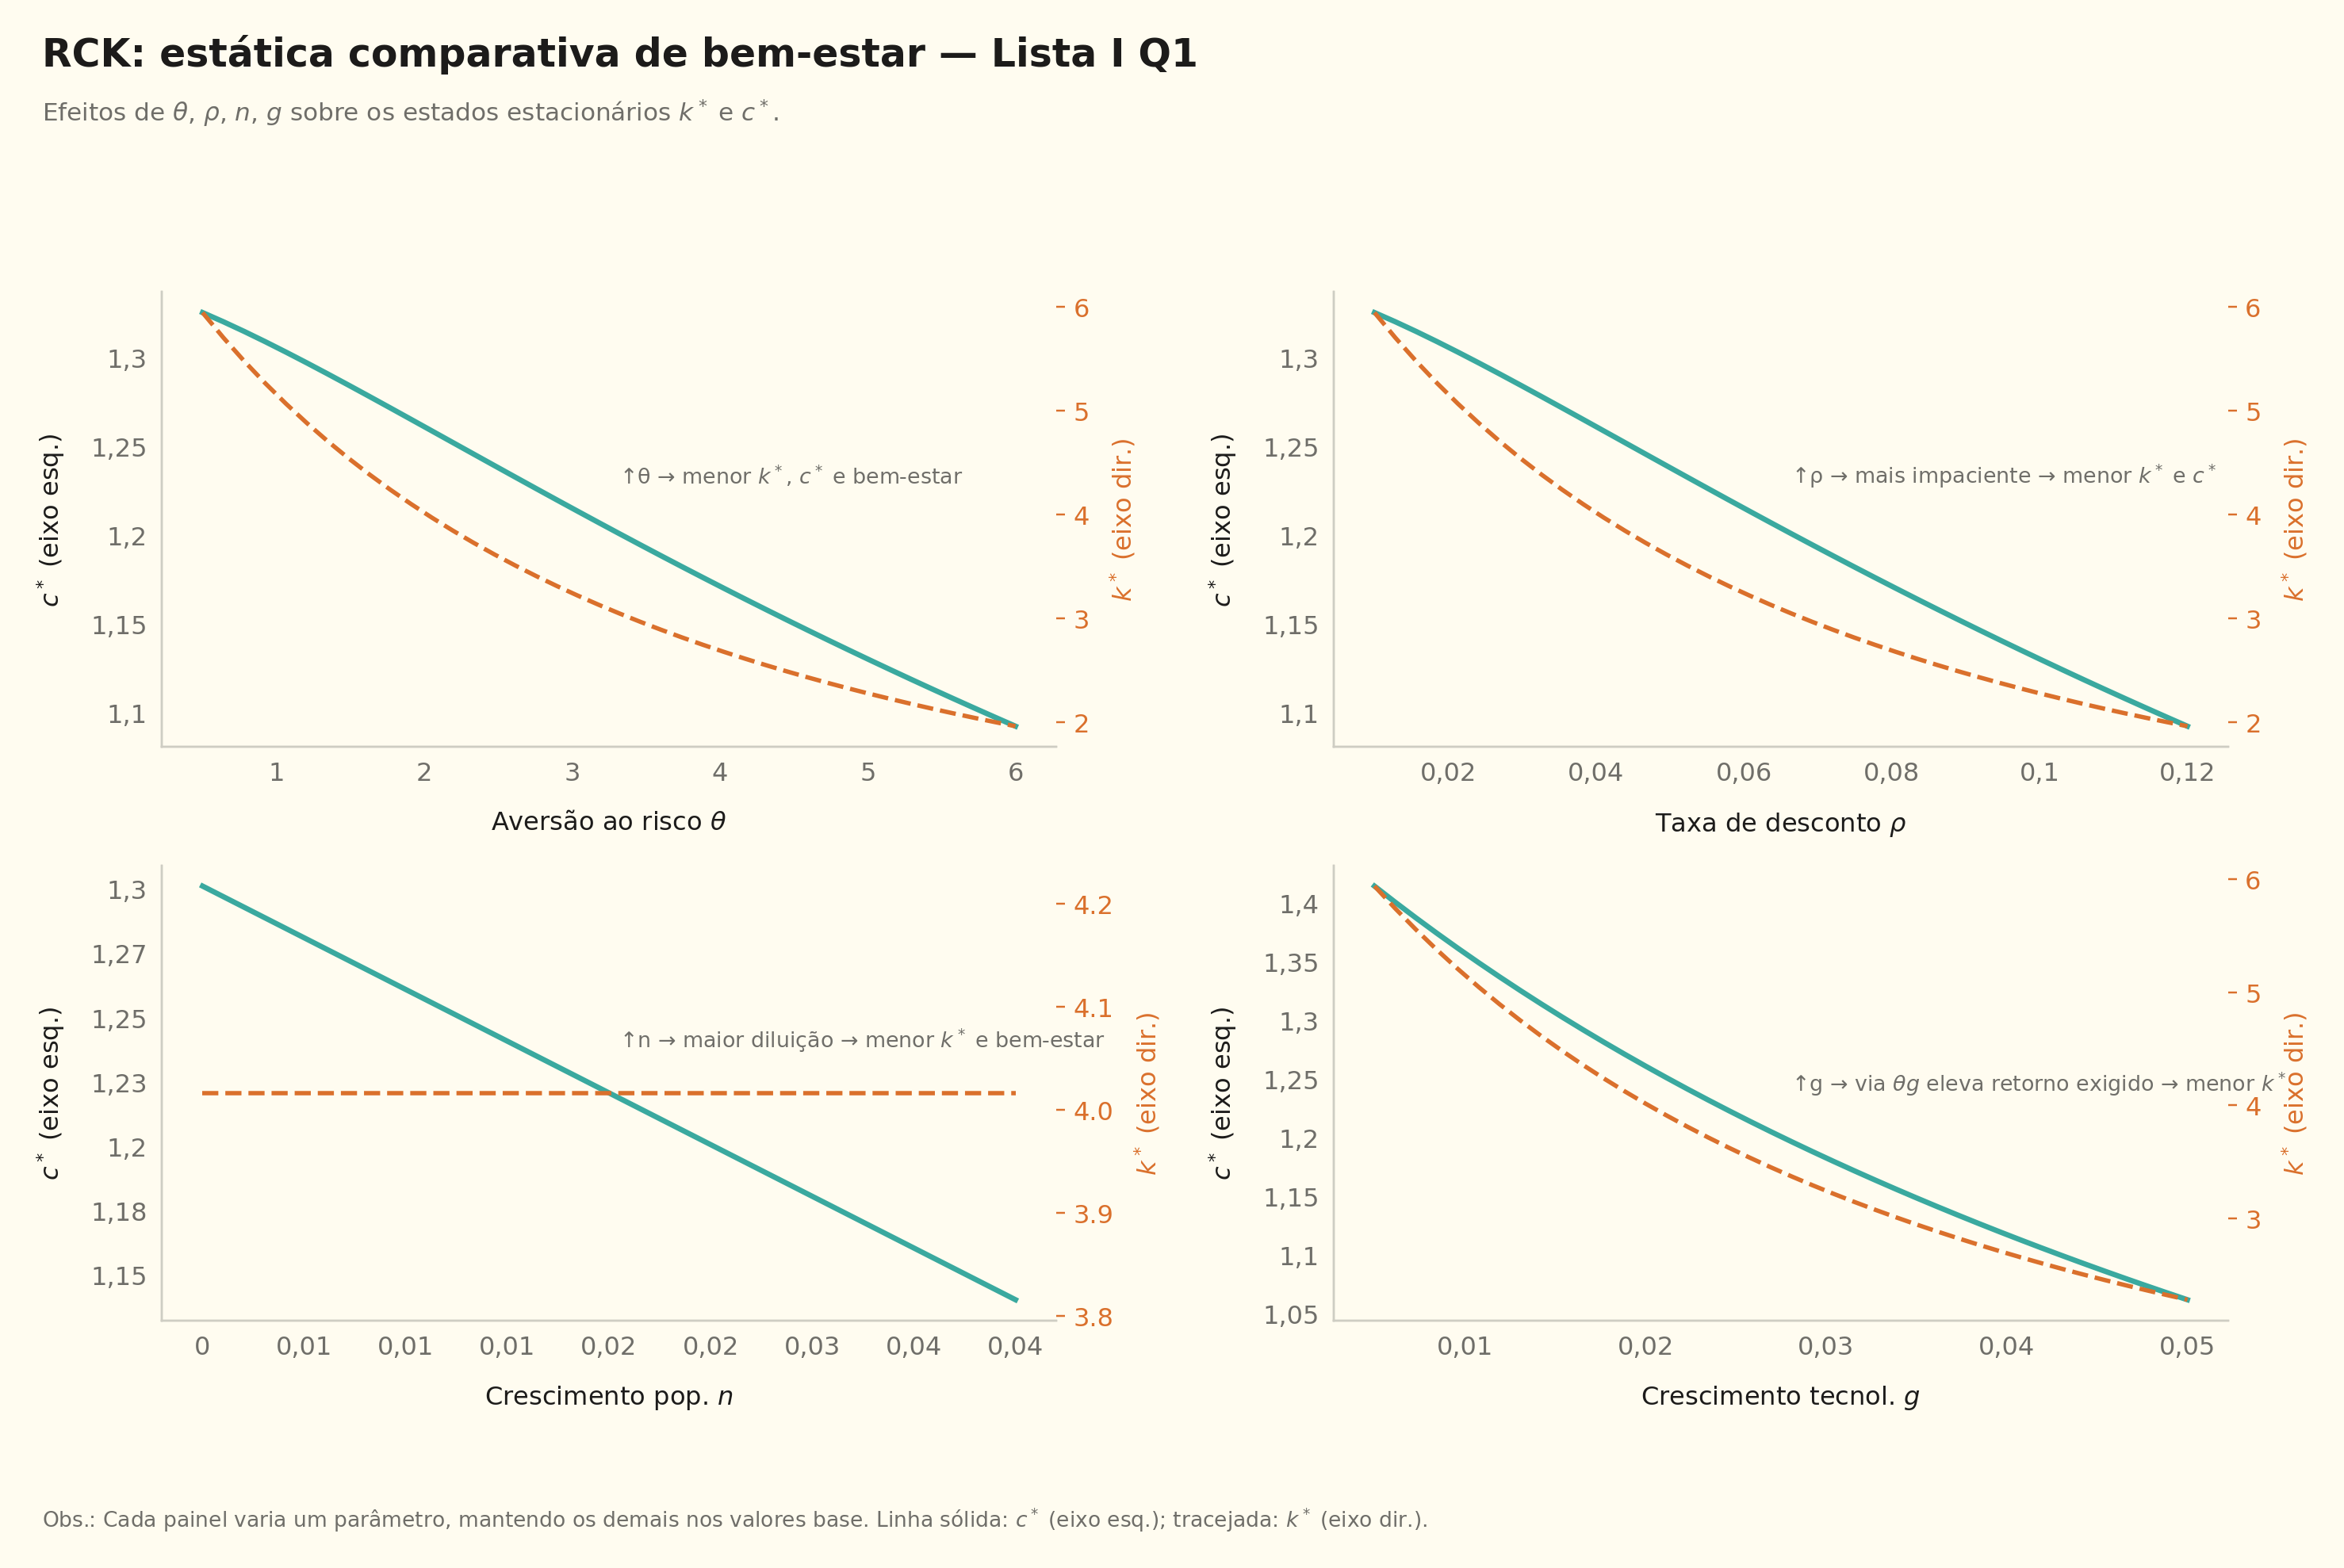
\includegraphics[width=0.85\textwidth]{rck_welfare_comparative.png}
\caption{Bem-estar $W^*$ em função dos parâmetros $\rho$, $\theta$, $n$ e $g$.}
\end{figure}

% ==========================================================================
\section{Equação de Keynes-Ramsey e condição de convergência}

\subsection*{Enunciado resumido}
Derive a equação de Euler do consumidor, interprete seus termos e deduza a condição
de convergência $\rho - n - (1-\theta)g > 0$.

% ------------------------------------------------------------------
\subsection*{2.1 \ Problema do consumidor}

O consumidor representativo maximiza:
\[
\max_{\{c(t)\}} \int_0^\infty u(c(t))\,e^{-(\rho-n)t}\,\dif t
\]
sujeito a $\dot{a}(t) = w(t) + r(t)\,a(t) - c(t) - n\,a(t)$,
onde $a(t)$ é a riqueza por pessoa adulta.

Hamiltoniano:
\[
H = e^{-(\rho-n)t}\,u(c) + \mu\bigl[w + ra - c - na\bigr].
\]
Condições de ótimo:
\begin{align}
\frac{\partial H}{\partial c} &= 0 \implies e^{-(\rho-n)t}\,u'(c) = \mu, \label{eq:foc_c}\\
\dot{\mu} &= -\frac{\partial H}{\partial a} \implies \dot{\mu} = -\mu(r - n). \label{eq:foc_mu}
\end{align}

% ------------------------------------------------------------------
\subsection*{2.2 \ Derivação da regra de Keynes-Ramsey}

Diferenciando \eqref{eq:foc_c} em relação ao tempo:
\[
-(\rho-n)\,e^{-(\rho-n)t}\,u'(c) + e^{-(\rho-n)t}\,u''(c)\,\dot{c} = \dot{\mu}.
\]
Usando \eqref{eq:foc_mu} e dividindo por $e^{-(\rho-n)t}\,u'(c)$:
\[
-(\rho-n) + \frac{u''(c)\,\dot{c}}{u'(c)} = -(r-n).
\]
Para CRRA, $u''(c)/u'(c)=-\theta/c$. Reorganizando:
\begin{equation}
\boxed{
\frac{\dot{c}}{c} = \frac{r - \rho}{\theta} = \frac{f'(k) - \delta - \rho}{\theta}.
}
\label{eq:keynes_ramsey}
\end{equation}

Em variáveis por unidade efetiva ($\tilde{c}=c/A$, com $\dot{A}/A=g$):
\[
\frac{\dot{\tilde{c}}}{\tilde{c}} = \frac{f'(\tilde{k}) - \delta - \rho - \theta g}{\theta}.
\]

% ------------------------------------------------------------------
\subsection*{2.3 \ Condição de convergência da integral de bem-estar}

\begin{formulabox}[title={Derivação da condição de transversalidade}]
O bem-estar intertemporal é:
\[
W = \int_0^\infty \frac{c(t)^{1-\theta}-1}{1-\theta}\,e^{-(\rho-n)t}\,\dif t.
\]
Ao longo da trajetória de crescimento equilibrado, $c(t)=c_0\,e^{gt}$, portanto:
\[
c(t)^{1-\theta} = c_0^{1-\theta}\,e^{(1-\theta)gt}.
\]
O integrando cresce como $e^{[(1-\theta)g - (\rho-n)]t}$. Para convergência:
\[
(1-\theta)g - (\rho-n) < 0
\implies \rho - n - (1-\theta)g > 0.
\]
Esta é também a condição de transversalidade:
$\lim_{t\to\infty} k(t)\mu(t)e^{-(\rho-n)t}=0$ exige que o capital não cresça mais
rápido que $(\rho-n)$, o que é garantido por esta desigualdade.
\end{formulabox}

\begin{provabox}[title={Atenção --- Cai na Prova (Q2 / P1 2024)}]
A P1 2024 apresentou a condição com \textbf{sinal trocado}: $\rho - n + (1-\theta)g > 0$
--- isso está \textbf{errado}. A condição correta é $\rho - n - (1-\theta)g > 0$.
Pontos-chave para a prova:
\begin{itemize}[leftmargin=1.5em, topsep=2pt, itemsep=2pt]
  \item $\rho$ tem efeito \textbf{negativo} sobre $\dot{c}/c$: impaciência freia crescimento.
  \item $1/\theta$ é a EIS: $\theta$ alto $\Rightarrow$ pouca resposta de consumo a $r$.
  \item No EE: $\dot{c}/c = 0 \Rightarrow r = \rho + \theta g$ (não $r=\rho$!).
  \item A condição de transversalidade ``mata'' trajetórias explosivas.
\end{itemize}
\end{provabox}

\begin{resultbox}[title={Interpretação da regra de Keynes-Ramsey}]
\begin{itemize}[leftmargin=1.5em, topsep=2pt, itemsep=2pt]
\item $r > \rho$: retorno $>$ impaciência $\Rightarrow$ adiar consumo $\Rightarrow$ $\dot{c}>0$.
\item $r < \rho$: impaciência domina $\Rightarrow$ $\dot{c}<0$.
\item EE: $r = \rho + \theta g$ garante $\dot{\tilde{c}}=0$.
\item $1/\theta$ é a \textbf{elasticidade de substituição intertemporal}.
\end{itemize}
\end{resultbox}

\begin{figure}[H]
\centering

\includegraphics[width=0.85\textwidth]{rck_phase_diagram.png}
\caption{Diagrama de fase do modelo RCK: curvas $\dot{k}=0$ e $\dot{c}=0$, equilíbrio
do tipo sela e trajetórias representativas.}
\end{figure}

% ==========================================================================
\section{Dinâmica do diagrama de fase: regiões e setas}

\subsection*{Enunciado resumido}
No diagrama de fase $(k, c)$, descreva a dinâmica na região à esquerda de $\dot{c}=0$
e acima de $\dot{k}=0$, e complete o mapa para todas as quatro regiões.

% ------------------------------------------------------------------
\subsection*{3.1 \ As duas curvas de lugar-zero}

\textbf{Locus $\dot{c}=0$} (linha vertical em $k=\kstar$):
\[
f'(k)-\delta = \rho + \theta g \implies k = \kstar.
\]
\begin{itemize}[leftmargin=1.5em, topsep=2pt, itemsep=1pt]
  \item À \textbf{esquerda}: $k < \kstar \Rightarrow f'(k) > \rho+\theta g \Rightarrow \dot{c}>0$.
  \item À \textbf{direita}: $k > \kstar \Rightarrow f'(k) < \rho+\theta g \Rightarrow \dot{c}<0$.
\end{itemize}

\textbf{Locus $\dot{k}=0$} (curva côncava):
\[
c = f(k) - (\delta+n+g)\,k.
\]
\begin{itemize}[leftmargin=1.5em, topsep=2pt, itemsep=1pt]
  \item \textbf{Acima}: consumo excessivo para a acumulação ser zero $\Rightarrow \dot{k}<0$.
  \item \textbf{Abaixo}: consumo insuficiente para zerar acumulação $\Rightarrow \dot{k}>0$.
\end{itemize}

% ------------------------------------------------------------------
\subsection*{3.2 \ Mapa completo das quatro regiões}

\begin{resultbox}[title={Diagrama de fases: quatro quadrantes}]
\begin{center}
\begin{tabular}{p{4.8cm}p{3.5cm}p{3.5cm}}
\toprule
Região & Sinal de $\dot{c}$ & Sinal de $\dot{k}$ \\
\midrule
Esq.\ de $\dot{c}=0$ e \textbf{acima} de $\dot{k}=0$
  & $\dot{c}>0$ ($c$ sobe) & $\dot{k}<0$ ($k$ cai) \\[4pt]
Esq.\ de $\dot{c}=0$ e \textbf{abaixo} de $\dot{k}=0$
  & $\dot{c}>0$ ($c$ sobe) & $\dot{k}>0$ ($k$ sobe) \\[4pt]
Dir.\ de $\dot{c}=0$ e \textbf{acima} de $\dot{k}=0$
  & $\dot{c}<0$ ($c$ cai) & $\dot{k}<0$ ($k$ cai) \\[4pt]
Dir.\ de $\dot{c}=0$ e \textbf{abaixo} de $\dot{k}=0$
  & $\dot{c}<0$ ($c$ cai) & $\dot{k}>0$ ($k$ sobe) \\
\bottomrule
\end{tabular}
\end{center}
\end{resultbox}

% ------------------------------------------------------------------
\subsection*{3.3 \ Região específica da Lista I Q3}

Na região \textit{esquerda de $\dot{c}=0$} e \textit{acima de $\dot{k}=0$}:

\begin{resultbox}[title={Dinâmica Q3: $\dot{c}>0$ e $\dot{k}<0$}]
\begin{center}
\begin{tabular}{p{4.5cm}p{4.5cm}p{2.8cm}}
\toprule
Condição & Equação & Direção \\
\midrule
$k < \kstar$ (esq.\ de $\dot{c}=0$) & $f'(k) > \rho + \theta g$ & $\dot{c}>0$: $c$ sobe \\[4pt]
$c > c_{\text{locus}}(k)$ (acima de $\dot{k}=0$) & consumo drena capital & $\dot{k}<0$: $k$ cai \\
\bottomrule
\end{tabular}
\end{center}
Trajetórias nesta região divergem para o noroeste e \textbf{não} convergem ao
equilíbrio --- violam a condição de transversalidade.
\end{resultbox}

\begin{provabox}[title={Atenção --- Cai na Prova (Q3 / Q4 P1 2024)}]
O diagrama de fases é cobrado diretamente em questões de múltipla escolha.
Memorize as regras:
\begin{itemize}[leftmargin=1.5em, topsep=2pt, itemsep=2pt]
  \item Esq.\ de $\dot{c}=0$: $f'(k)$ alto $\Rightarrow$ retorno $>$ desconto $\Rightarrow$ $\dot{c}>0$.
  \item Dir.\ de $\dot{c}=0$: oposto.
  \item Acima de $\dot{k}=0$: muito consumo $\Rightarrow$ capital cai.
  \item Abaixo de $\dot{k}=0$: pouco consumo $\Rightarrow$ capital acumula.
\end{itemize}
Questão-tipo P1 2024 (Apêndice Q-tipo 4): ``à direita de $\dot{c}=0$ e abaixo de
$\dot{k}=0$'' $\Rightarrow$ $\dot{c}<0$ e $\dot{k}>0$.
\end{provabox}

\begin{figure}[H]
\centering

\includegraphics[width=0.85\textwidth]{rck_phase_diagram.png}
\caption{Diagrama de fase do modelo RCK. Região Q3 (esq.\ de $\dot{c}=0$, acima de
$\dot{k}=0$): setas apontam para noroeste ($\dot{c}>0$, $\dot{k}<0$).}
\end{figure}

% ==========================================================================
%  PARTE II — MODELO RBC (Questões 4-8)
% ==========================================================================

\newpage
\section*{\large\color{cyanrbc} Parte II --- Modelo de Ciclos Reais de Negócios (Q4--Q8)}
\addcontentsline{toc}{section}{Parte II --- Modelo RBC (Q4--Q8)}

O modelo RBC de tempo discreto (Romer, cap.\ 5) incorpora choques de PTF $z_t$
seguindo AR(1):
\[
\log z_{t+1} = \rho_z \log z_t + \varepsilon_{t+1}, \quad
\varepsilon \sim \mathcal{N}(0,\sigma_z^2).
\]
Produção: $Y_t = z_t K_t^\alpha$. Acumulação: $K_{t+1} = (1-\delta)K_t + I_t$.

% ==========================================================================
\section{Estabilidade do capital no estado estacionário}

\subsection*{Enunciado resumido}
Demonstre que $I^*=\delta K^*$ no estado estacionário do modelo RBC e que $|A|<1$
(estabilidade dinâmica).

% ------------------------------------------------------------------
\subsection*{4.1 \ Condição de estado estacionário para o capital}

No EE, $z_t=1$ e $K_{t+1}=K_t=\kstar$:
\[
K_{t+1} - K_t = I_t - \delta K_t = 0 \implies I^* = \delta\kstar.
\]

\begin{resultbox}[title={Interpretação de $I^*=\delta K^*$}]
No estado estacionário, o investimento líquido é zero: toda a poupança serve apenas
para repor o capital depreciado. É a condição de estacionariedade do estoque de capital.
\end{resultbox}

% ------------------------------------------------------------------
\subsection*{4.2 \ Equação de Euler e taxa de retorno}

Equação de Fisher/Ramsey discreta:
\[
\frac{1}{C_t} = \beta\,\E_t\!\left[\frac{r_{t+1}+1-\delta}{C_{t+1}}\right].
\]
No EE ($C_{t+1}=C_t=\cstar$):
\begin{equation}
\beta(\rstar+1-\delta) = 1 \implies
\rstar = \frac{1}{\beta}-(1-\delta) = \frac{1-\beta(1-\delta)}{\beta}.
\label{eq:rstar_rbc}
\end{equation}
Para $\beta=0.99$, $\delta=0.025$: $\rstar\approx 0.035$.

% ------------------------------------------------------------------
\subsection*{4.3 \ Estabilidade dinâmica via log-linearização}

Lei de movimento log-linearizada:
\[
\khat_{t+1} = A\,\khat_t + B\,\zhat_t, \quad A = \gamma_k - \gamma_c\,a_k.
\]
A raiz $|A|<1$ é selecionada pelo método dos coeficientes indeterminados.
Com parâmetros calibrados: $a_k\approx 0.590$, $A\approx 0.962 < 1$.

\begin{table}[H]
\centering
\caption{Valores calibrados para o modelo RBC padrão.}
\begin{tabular}{lll}
\toprule
Parâmetro & Valor & Definição \\
\midrule
$\alpha$ & 0.33 & Participação do capital \\
$\beta$ & 0.99 & Fator de desconto \\
$\delta$ & 0.025 & Taxa de depreciação \\
$\rho_z$ & 0.95 & Persistência do choque de PTF \\
$a_k$ & 0.590 & Coef.\ de consumo em capital \\
$A$ & 0.962 & Raiz da lei de movimento \\
\bottomrule
\end{tabular}
\end{table}

\begin{provabox}[title={Atenção --- Cai na Prova (Q4 / P1 2024 Q2 adaptado)}]
Na P1 2024, questões sobre RBC testaram:
\begin{itemize}[leftmargin=1.5em, topsep=2pt, itemsep=2pt]
  \item A condição de estabilidade é $|A|<1$ --- não $A=1$ (raiz unitária significa
    sem convergência).
  \item $I^*=\delta K^*$ é a condição de estado estacionário do capital --- a resposta
    correta para questão-tipo b) do Apêndice.
  \item $\beta(r^*+1-\delta)=1$ (a versão correta é com $r^*+1-\delta$, não $r^*-1+\delta$
    ou $r^*-\delta$).
\end{itemize}
\end{provabox}

\begin{figure}[H]
\centering
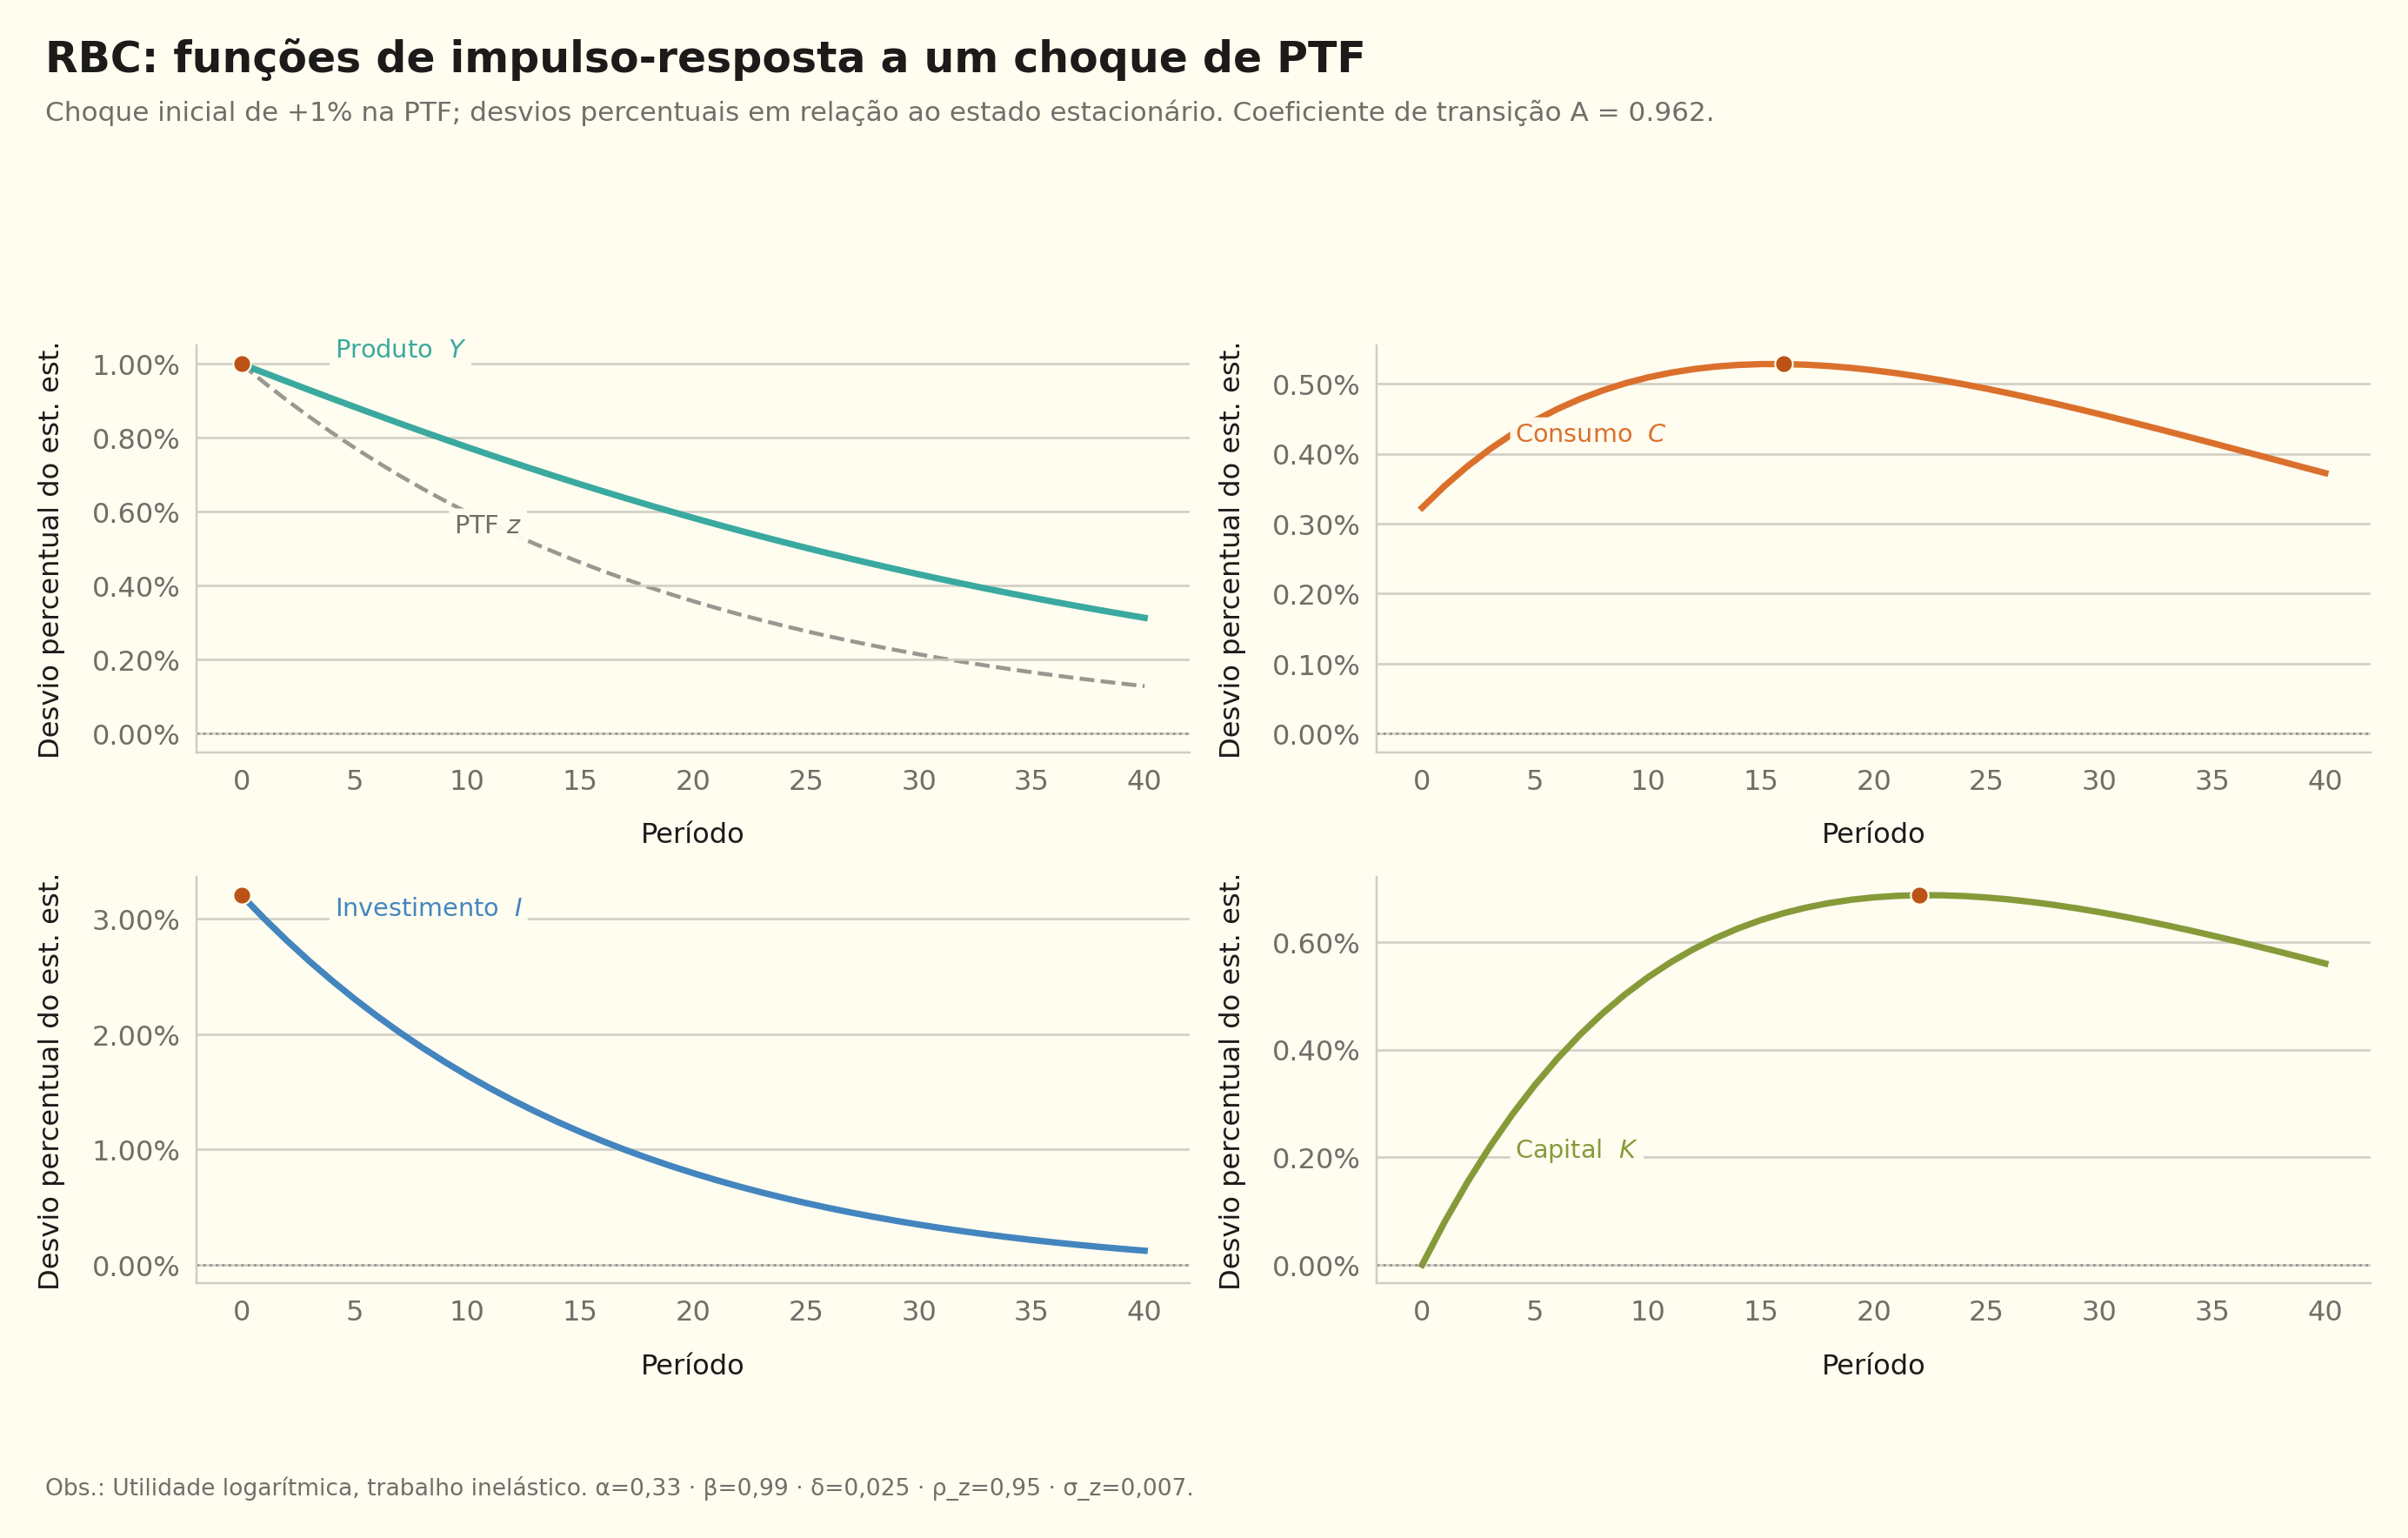
\includegraphics[width=0.85\textwidth]{rbc_irf.png}
\caption{Função de resposta ao impulso (FRI) do modelo RBC a um choque de 1\% de PTF.}
\end{figure}

\begin{figure}[H]
\centering
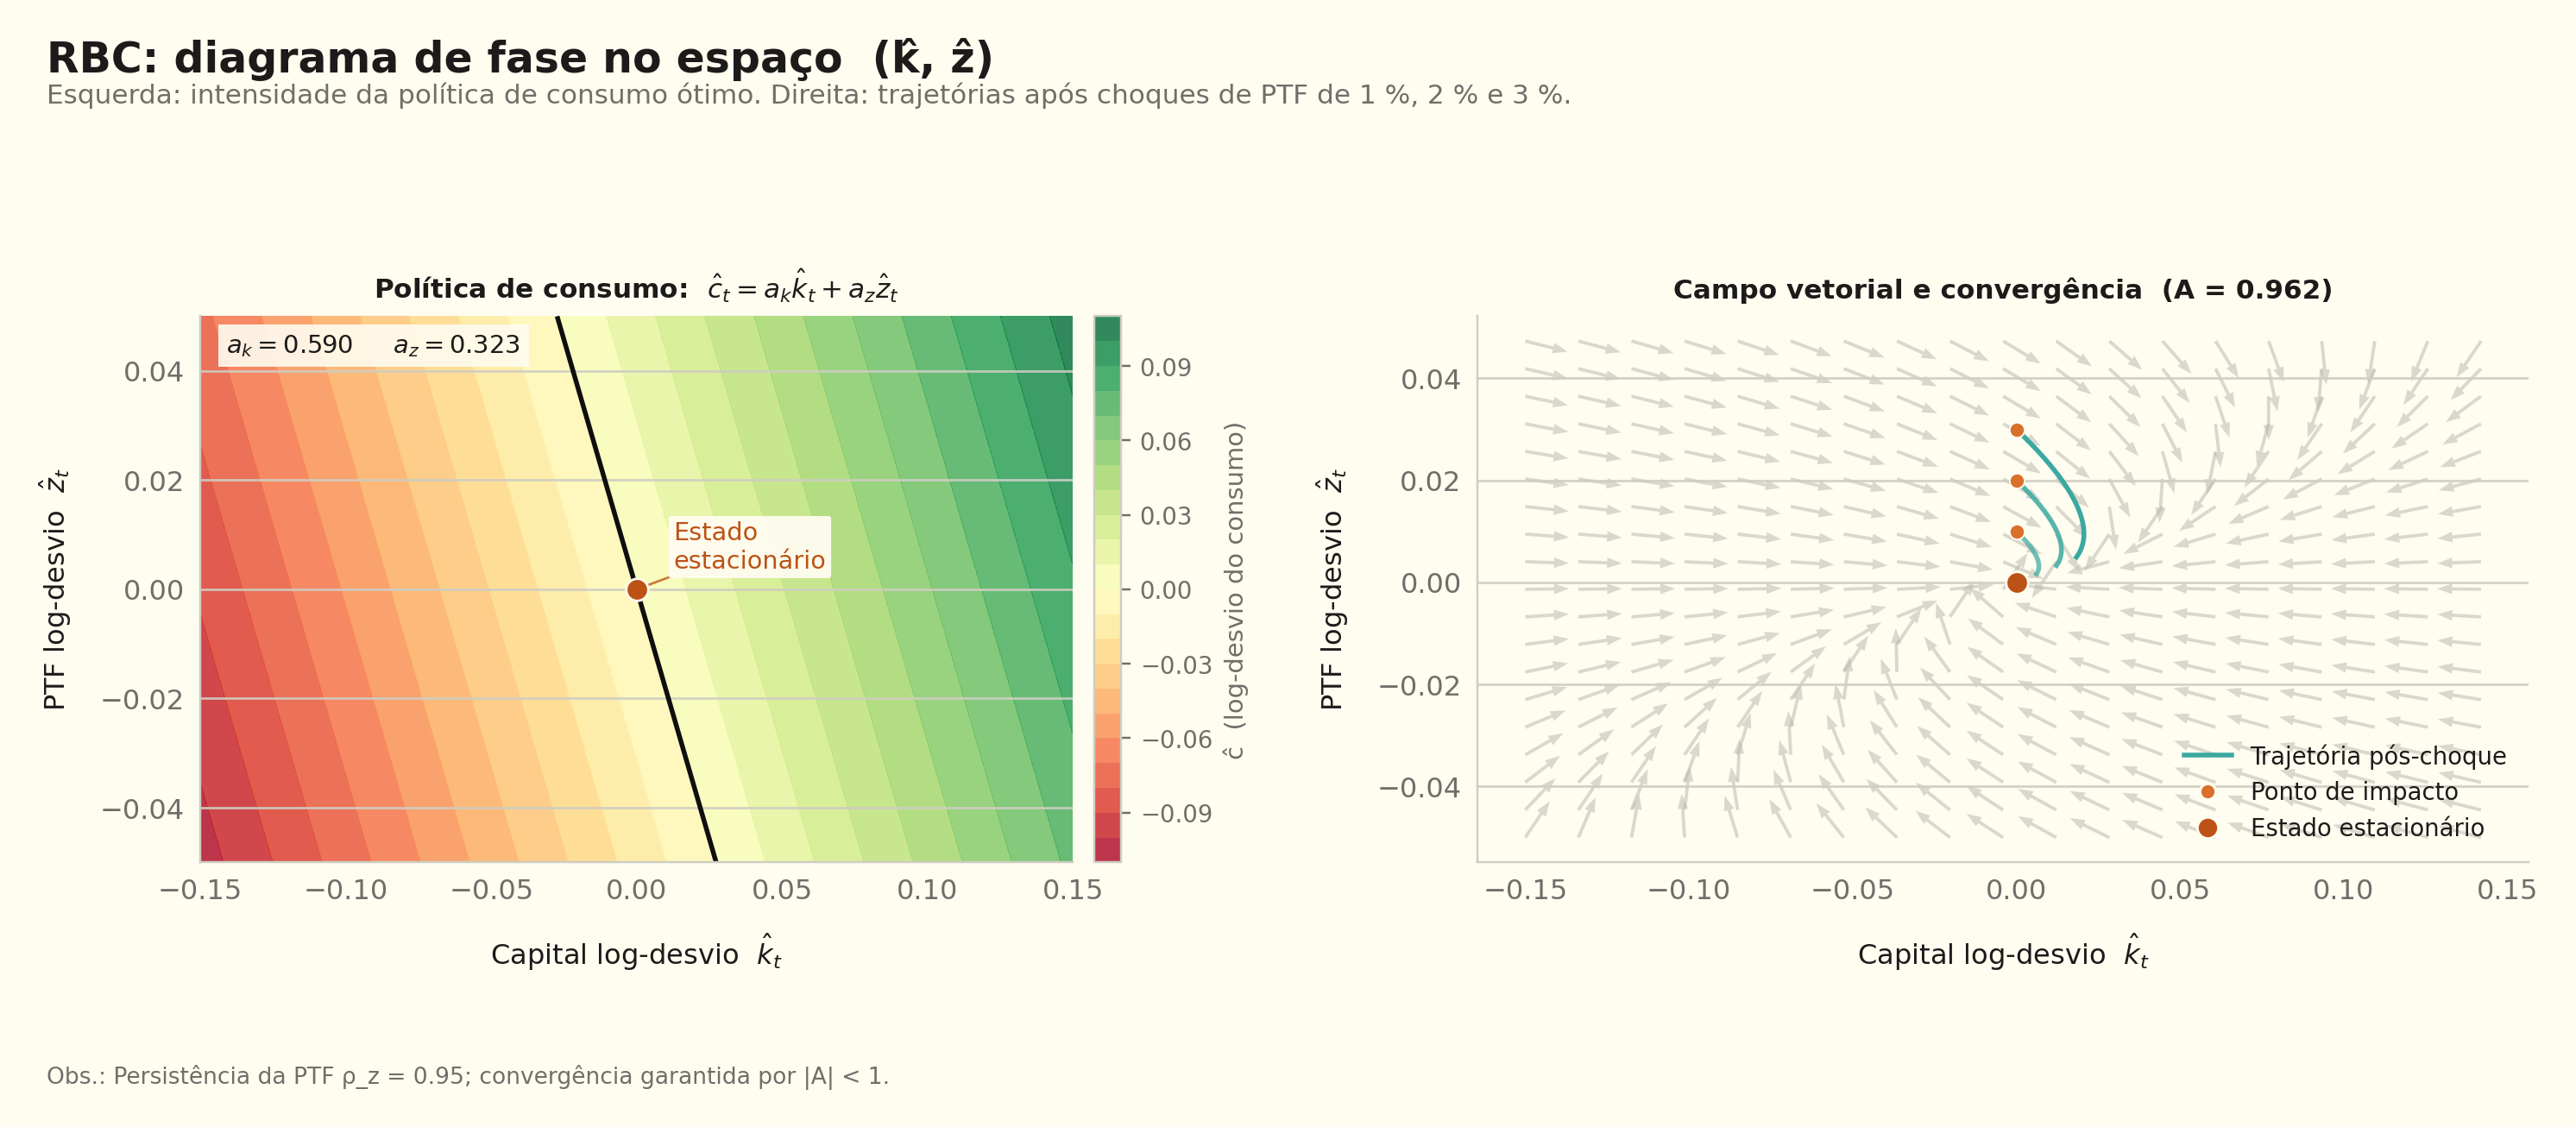
\includegraphics[width=0.85\textwidth]{rbc_phase_diagram.png}
\caption{Diagrama de fase do modelo RBC: trajetórias convergindo ao estado estacionário.}
\end{figure}

% ==========================================================================
\section{Desutilidade marginal do trabalho e oferta de trabalho alternativa}

\subsection*{Enunciado resumido}
Derive a desutilidade marginal do trabalho na versão com lazer do modelo RBC,
e apresente a fórmula alternativa de oferta de trabalho $U=C-(1/\eta)L^\eta$.

% ------------------------------------------------------------------
\subsection*{5.1 \ Utilidade com lazer}

\[
u(C_t, l_t) = \ln C_t + b\,\ln l_t, \quad b>0, \quad l_t = 1-N_t.
\]

% ------------------------------------------------------------------
\subsection*{5.2 \ Desutilidade marginal do trabalho (DML)}

Oferecer uma hora adicional de trabalho reduz $l_t$ em uma unidade:
\[
\frac{\partial(-u)}{\partial N_t}
= -\frac{\partial(b\ln l_t)}{\partial l_t}\cdot\frac{\partial l_t}{\partial N_t}
= \frac{b}{l_t}\cdot 1
= \frac{b}{1-N_t}.
\]

\begin{resultbox}[title={Desutilidade marginal do trabalho (Q5)}]
\[
\text{DML} = \frac{b}{1-N_t} = \frac{b}{l_t}.
\]
Crescente em $N_t$: quanto mais se trabalha, mais custosa cada hora extra.
Reflete o \textbf{valor marginal crescente do lazer}.
\end{resultbox}

% ------------------------------------------------------------------
\subsection*{5.3 \ Especificação alternativa: $U=C-(1/\eta)L^\eta$}

\begin{formulabox}[title={Derivação da oferta de trabalho com desutilidade polinomial (P1 2024 Q5)}]
Esta especificação apareceu na questão dissertativa da P1 2024.
Considere utilidade $U = C - \frac{1}{\eta}L^\eta$ com $\eta > 1$.
A CPO em relação a $L$ (dado salário real $W/P$):
\[
\frac{\partial U}{\partial C}\cdot\frac{W}{P} + \frac{\partial U}{\partial L} = 0
\implies 1\cdot\frac{W}{P} - L^{\eta-1} = 0.
\]
Resolvendo para $L^*$:
\[
L^{\eta-1} = \frac{W}{P}
\implies
\boxed{L^* = \left(\frac{W}{P}\right)^{1/(\eta-1)}}.
\]
\textbf{Interpretação}: a oferta de trabalho é crescente no salário real $W/P$
com elasticidade $1/(\eta-1)$. Para $\eta=2$: $L^*=W/P$ (linear). Para $\eta\to\infty$:
oferta inelástica ($L^*\to 1$ independente do salário).
\end{formulabox}

\begin{provabox}[title={Atenção --- Cai na Prova (Q5 dissertativa P1 2024)}]
Esta derivação apareceu explicitamente na questão dissertativa da P1 2024.
Passos exigidos:
\begin{enumerate}[leftmargin=1.5em, topsep=2pt, itemsep=2pt]
  \item Escrever a CPO: $W/P = L^{\eta-1}$.
  \item Isolar $L^*$: elevar ambos os lados a $1/(\eta-1)$.
  \item Interpretar: elasticidade da oferta de trabalho = $1/(\eta-1)$.
\end{enumerate}
Confundir $\eta$ com a elasticidade diretamente é erro comum --- a elasticidade
é $\mathbf{1/(\eta-1)}$, não $\eta$.
\end{provabox}

\begin{figure}[H]
\centering
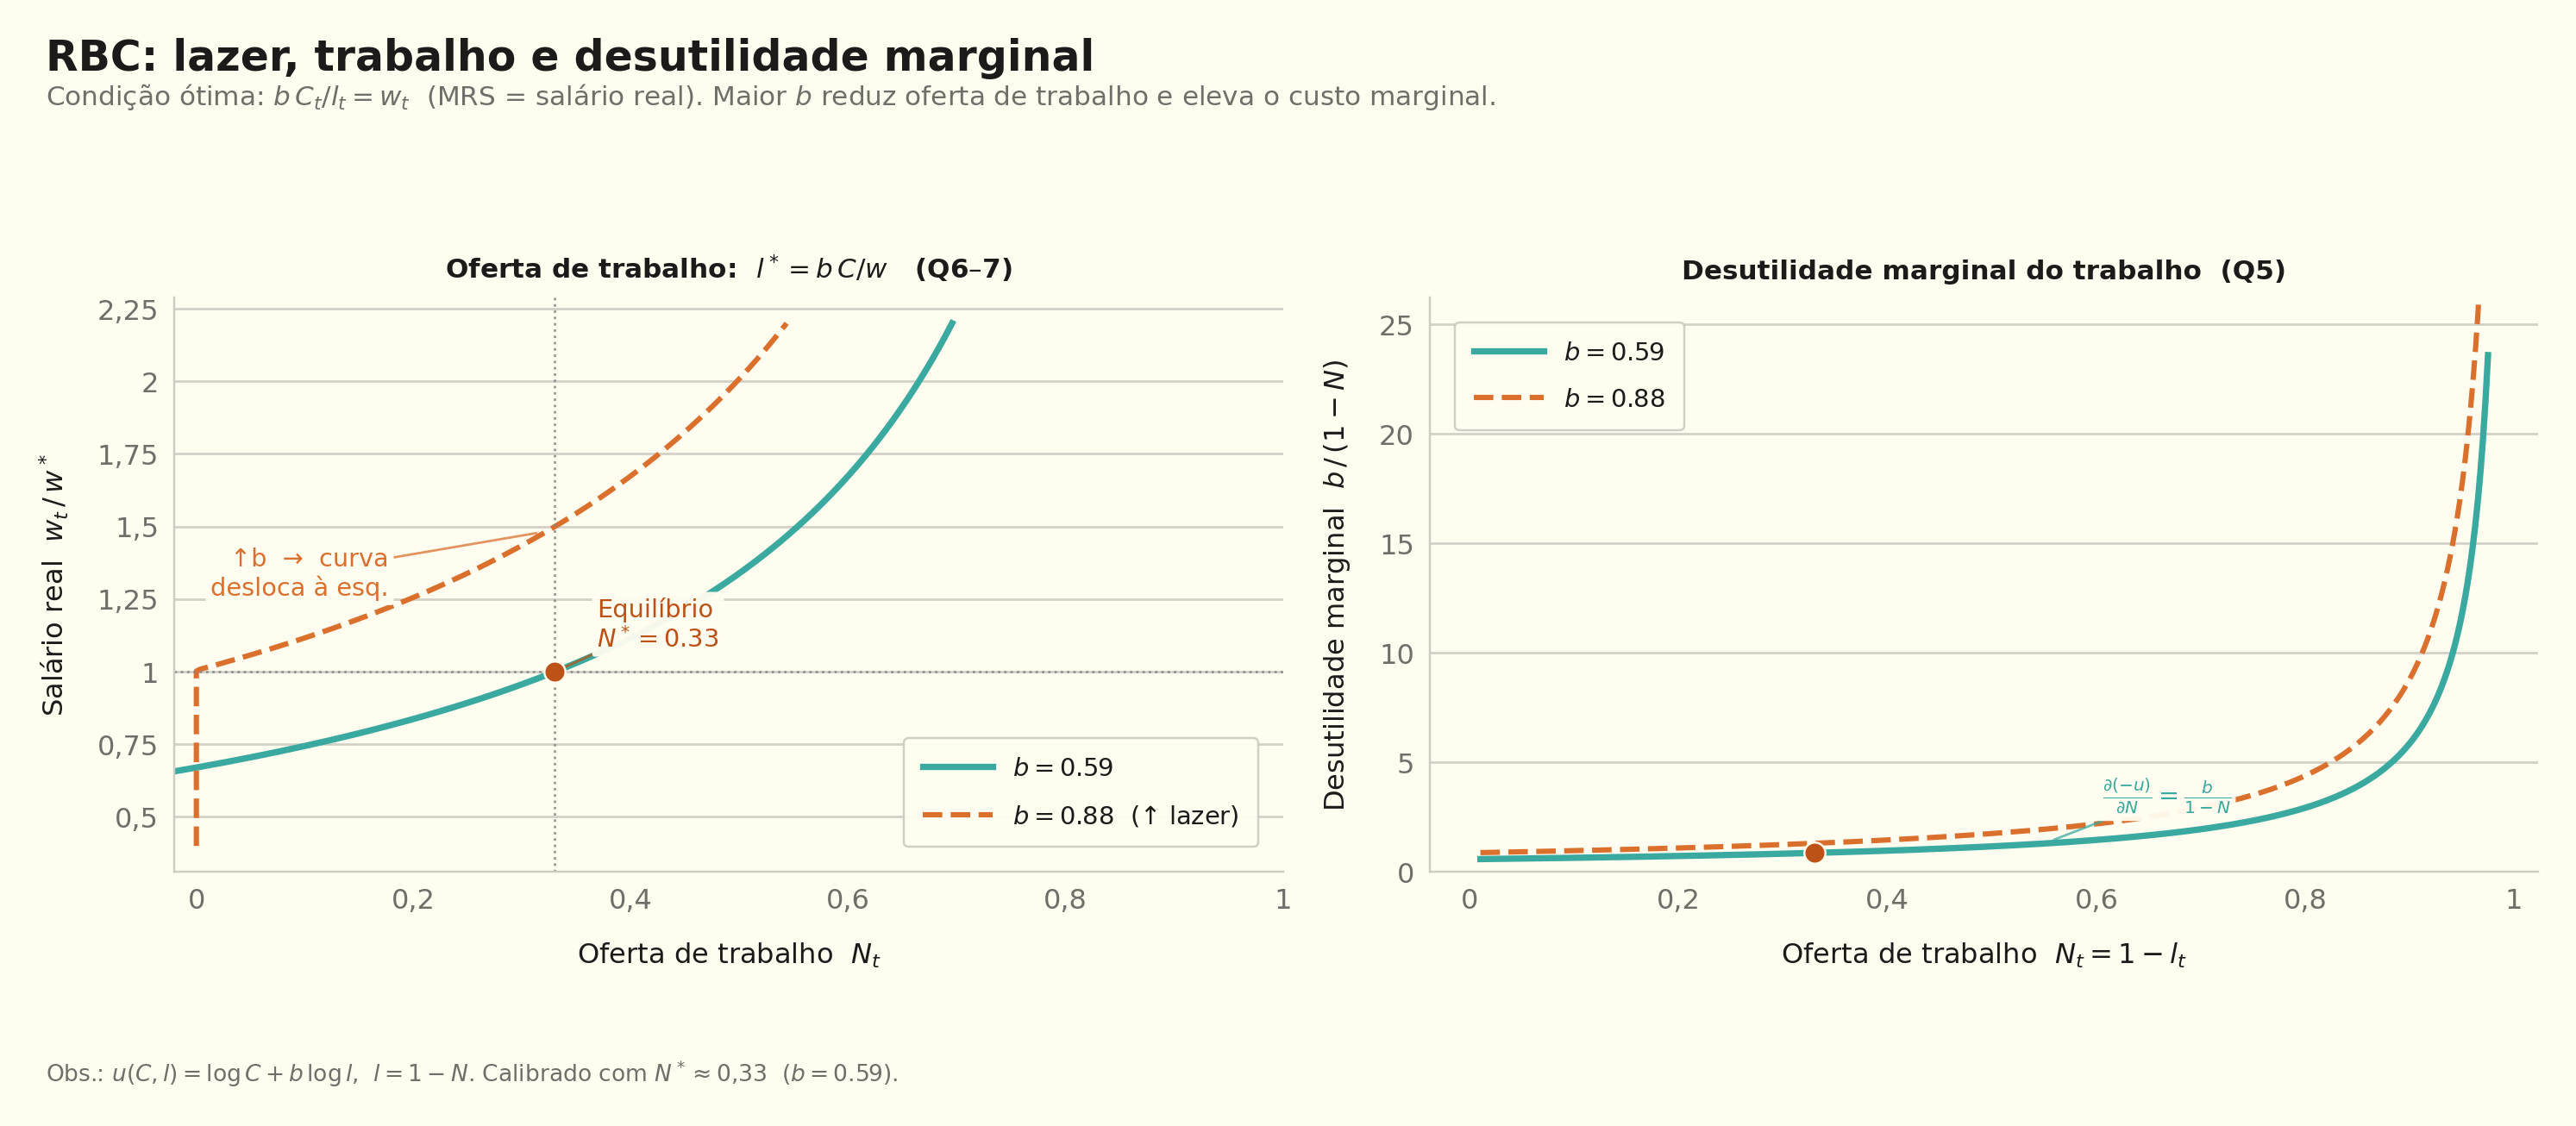
\includegraphics[width=0.85\textwidth]{rbc_labor_leisure.png}
\caption{Esquerda: oferta de trabalho em função do salário para diferentes $b$.
Direita: DML em função de $N=1-l$.}
\end{figure}

% ==========================================================================
\section{Resposta do lazer a variações na taxa de juros e salário futuro}

\subsection*{Enunciado resumido}
Como o lazer ótimo $l_t^*$ responde a $r_t\uparrow$ e a $w_{t+1}\uparrow$?
Derive a fórmula de substituição intertemporal de trabalho.

% ------------------------------------------------------------------
\subsection*{6.1 \ Condição de ótimo intratemporal}

Da maximização de $u(C,l)$ com $\partial u/\partial l = bC/l = w_t\cdot\partial u/\partial C$:
\[
\frac{b/l_t}{1/C_t} = \frac{bC_t}{l_t} = w_t
\implies
l_t^* = \frac{b\,C_t}{w_t}.
\]

% ------------------------------------------------------------------
\subsection*{6.2 \ Efeito de $r_t\uparrow$: lazer diminui}

Aumento em $r_t$:
\begin{enumerate}[leftmargin=1.5em, topsep=2pt, itemsep=2pt]
  \item Euler: $C_t$ cai (poupança mais atrativa).
  \item Com $w_t$ inalterado: $l_t^* = bC_t/w_t$ \textbf{diminui}.
  \item $N_t = 1-l_t^*$ sobe: o trabalhador substitui lazer hoje por lazer amanhã.
\end{enumerate}

\begin{resultbox}[title={Lazer e taxa de juros (Q6a)}]
$r_t\uparrow$ $\Rightarrow$ $C_t\downarrow$ (substituição intertemporal de consumo)
$\Rightarrow$ $l_t^*\downarrow$ (menos lazer) $\Rightarrow$ $N_t\uparrow$ (mais trabalho hoje).
\end{resultbox}

% ------------------------------------------------------------------
\subsection*{6.3 \ Efeito de $w_{t+1}\uparrow$: lazer aumenta}

Aumento antecipado em $w_{t+1}$ (efeito riqueza via Euler):
\begin{enumerate}[leftmargin=1.5em, topsep=2pt, itemsep=2pt]
  \item Consumidor se sente mais rico; $C_t$ sobe.
  \item Com $w_t$ fixo: $l_t^* = bC_t/w_t$ \textbf{aumenta}.
  \item O trabalhador descansa mais hoje na antecipação de salários futuros altos.
\end{enumerate}

\begin{resultbox}[title={Lazer e salário futuro (Q6b)}]
$w_{t+1}\uparrow$ $\Rightarrow$ efeito riqueza positivo $\Rightarrow$ $C_t\uparrow$
$\Rightarrow$ $l_t^*\uparrow$ (mais lazer) $\Rightarrow$ $N_t\downarrow$ (menos trabalho hoje).
\end{resultbox}

% ------------------------------------------------------------------
\subsection*{6.4 \ Fórmula da substituição intertemporal de trabalho}

\begin{formulabox}[title={Derivação da equação de substituição intertemporal (P1 2024 Q2)}]
A condição intratemporal em $t$ e $t+1$:
\[
\frac{bC_t}{l_t} = w_t \quad\text{e}\quad \frac{bC_{t+1}}{l_{t+1}} = w_{t+1}.
\]
A equação de Euler intertemporal de consumo:
\[
\frac{1}{C_t} = \beta(1+r)\frac{1}{C_{t+1}} \implies C_{t+1} = \beta(1+r)C_t.
\]
Substituindo na condição de $t+1$:
\[
\frac{b\beta(1+r)C_t}{l_{t+1}} = w_{t+1}
\implies l_{t+1} = \frac{b\beta(1+r)C_t}{w_{t+1}}.
\]
Dividindo $l_t/l_{t+1}$:
\[
\frac{l_t}{l_{t+1}} = \frac{bC_t/w_t}{b\beta(1+r)C_t/w_{t+1}}
= \frac{w_{t+1}}{\beta(1+r)w_t}.
\]
Reescrevendo em termos de trabalho $N_i = 1-l_i$... em notação compacta:
\begin{equation}
\boxed{
\frac{1-l_1}{1-l_2} = \beta(1+r)\frac{w_2}{w_1}.
}
\label{eq:intertemporal_labor}
\end{equation}
\end{formulabox}

\begin{provabox}[title={Atenção --- Cai na Prova (Q2 / P1 2024)}]
A fórmula $\dfrac{1-l_1}{1-l_2} = \beta(1+r)\dfrac{w_2}{w_1}$ foi testada
\textbf{diretamente} na P1 2024 Q2. Interpretação:
\begin{itemize}[leftmargin=1.5em, topsep=2pt, itemsep=2pt]
  \item $r\uparrow$ $\Rightarrow$ lado direito $\uparrow$ $\Rightarrow$ $N_1/N_2\uparrow$:
    mais trabalho hoje relativamente ao futuro.
  \item $w_2\uparrow$ (com $w_1$ fixo): lado direito $\uparrow$ $\Rightarrow$ $N_1\uparrow$
    --- efeito substituição puro (trabalha hoje quando lazer amanhã é mais caro).
  \item A alternativa errada da P1 2024 dizia: ``$r\uparrow$ reduz oferta de trabalho
    presente'' --- o contrário do correto.
\end{itemize}
\end{provabox}

% ==========================================================================
\section{Razão consumo-lazer e calibração de \texorpdfstring{$b$}{b}}

\subsection*{Enunciado resumido}
Derive a razão $C/l$ e calibre $b$ usando dados de horas trabalhadas.

% ------------------------------------------------------------------
\subsection*{7.1 \ Razão ótima \texorpdfstring{$C/l$}{C/l}}

Da condição intratemporal:
\begin{equation}
\frac{C_t}{l_t^*} = \frac{w_t}{b}.
\label{eq:cl_ratio}
\end{equation}
Intuição: salário alto $\Rightarrow$ lazer caro $\Rightarrow$ razão $C/l$ alta
(consome relativamente mais, descansa relativamente menos); $b$ alto $\Rightarrow$
lazer preferido $\Rightarrow$ razão $C/l$ baixa.

% ------------------------------------------------------------------
\subsection*{7.2 \ Calibração de \texorpdfstring{$b$}{b}}

Fração de horas trabalhadas no EE: $N^*=1/3$, logo $l^*=2/3$.
No EE: $w^* = (1-\alpha)(\kstar)^\alpha = (1-\alpha)y^*/N^*$.
De \eqref{eq:cl_ratio}:
\[
b = \frac{w^*\,l^*}{C^*} = \frac{w^*(1-N^*)}{C^*}.
\]
Para $\alpha=0.33$, $\kstar\approx 28.35$: $b\approx 1.55$.

\begin{provabox}[title={Atenção --- Cai na Prova (Q7)}]
A questão 7 da Lista I testa diretamente a manipulação algébrica de $C/l = w/b$.
Passos para a calibração:
\begin{enumerate}[leftmargin=1.5em, topsep=2pt, itemsep=2pt]
  \item Isolar $b$: $b = wl/C = w(1-N)/C$.
  \item Substituir valores de EE: $w^*$, $l^*=1-N^*$, $C^*$.
  \item Calcular numericamente.
\end{enumerate}
Se a questão perguntar ``qual o efeito de $b\uparrow$ sobre $N^*$?'':
$b\uparrow \Rightarrow l^*\uparrow \Rightarrow N^*\downarrow$ (menos trabalho).
\end{provabox}

\begin{figure}[H]
\centering
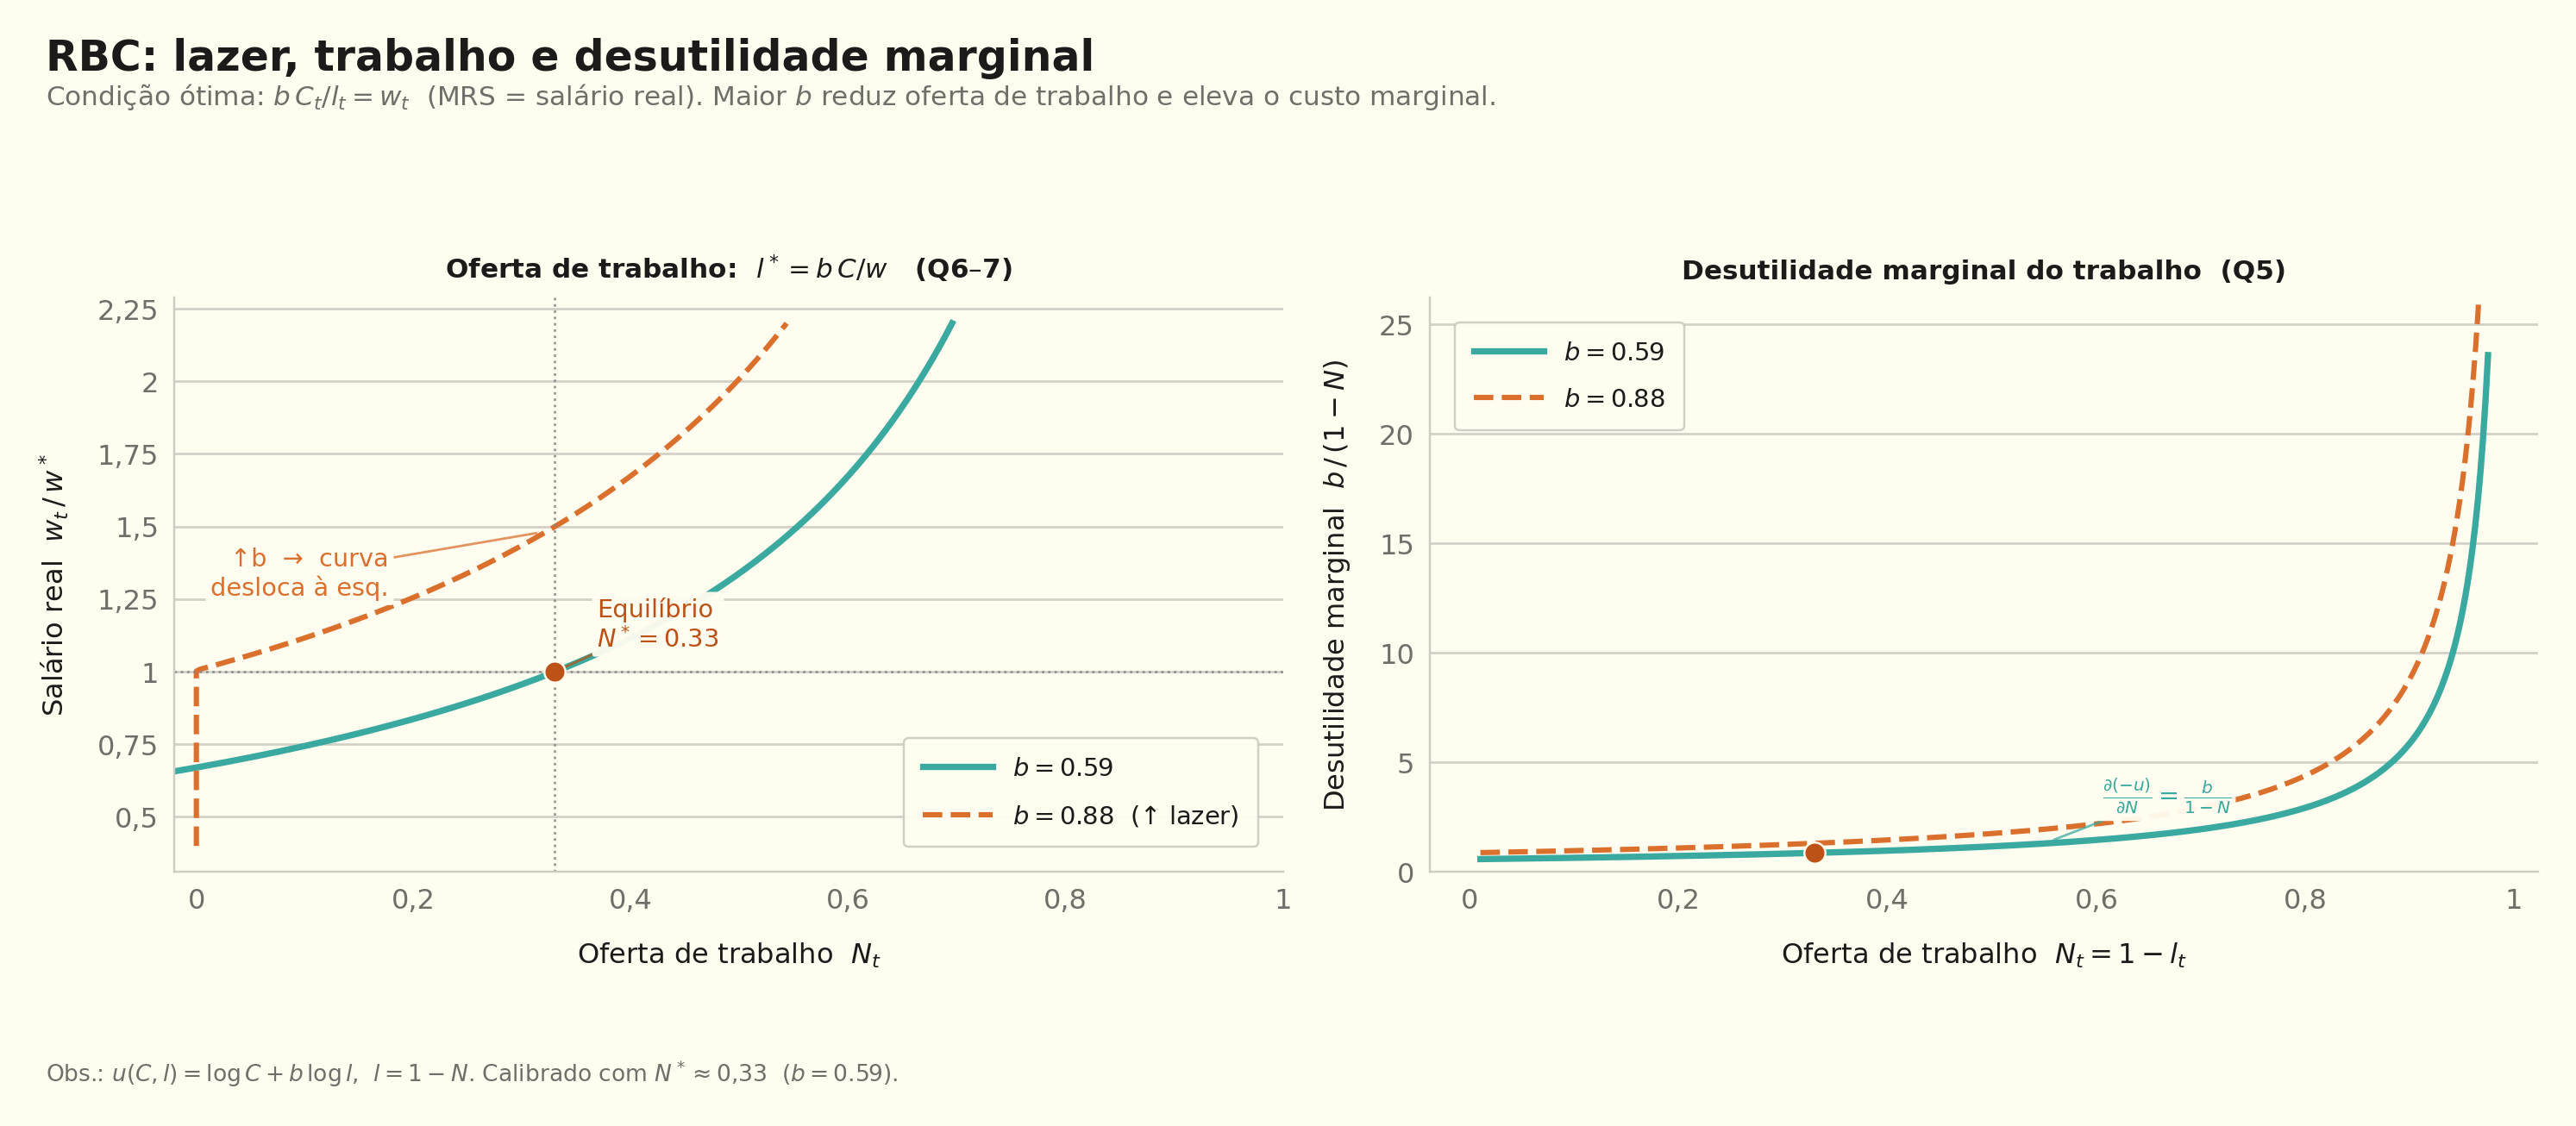
\includegraphics[width=0.85\textwidth]{rbc_labor_leisure.png}
\caption{Oferta de trabalho para diferentes $b$; linha tracejada: equilíbrio $N^*=1/3$.}
\end{figure}

% ==========================================================================
\section{Três canais de transmissão de choques de PTF}

\subsection*{Enunciado resumido}
Explique os mecanismos pelos quais $z_t\uparrow$ afeta a economia e conecte ao canal
de oferta de trabalho e substituição intertemporal.

% ------------------------------------------------------------------
\subsection*{8.1 \ O choque de PTF}

Um choque positivo $\varepsilon_t>0$ eleva $\log z_t$; impacto imediato:
\[
\hat{Y}_t = \hat{z}_t + \alpha\hat{K}_t
\xrightarrow{\hat{K}_t=0\text{ (período 0)}} \hat{Y}_0 = \hat{z}_0 = 1\%.
\]

% ------------------------------------------------------------------
\subsection*{8.2 \ Canal 1 --- Efeito direto na produção}

$z_t\uparrow$ eleva diretamente a produtividade de cada unidade de capital.
\textbf{Impacto}: $\hat{Y}_0 = 1\%$ exatamente (FRI confirma).

% ------------------------------------------------------------------
\subsection*{8.3 \ Canal 2 --- Amplificação do investimento}

A melhora esperada eleva a riqueza permanente; pela Euler, parte é poupada:
\[
\hat{I}_0 > \hat{Y}_0 \quad (\hat{I}_0 \approx 3.2\%).
\]
Capital acumulado $K_{t+1}$ sobe, amplificando produto nos períodos seguintes.

% ------------------------------------------------------------------
\subsection*{8.4 \ Canal 3 --- Suavização do consumo}

Aversão ao risco leva o consumidor a distribuir o ganho ao longo do tempo:
\[
\hat{C}_0 < \hat{Y}_0 \quad (\hat{C}_0 \approx 0.33\%).
\]
Implicação: $\sigma(C) < \sigma(Y)$ nas simulações.

% ------------------------------------------------------------------
\subsection*{8.5 \ Canal adicional: oferta de trabalho (substituição intertemporal)}

\begin{formulabox}[title={Canal da oferta de trabalho}]
Um choque de PTF também age sobre \textbf{horas trabalhadas} via substituição
intertemporal de trabalho:
\begin{enumerate}[leftmargin=1.5em, topsep=2pt, itemsep=2pt]
  \item $z_t\uparrow$ eleva $w_t = (1-\alpha)z_t K_t^\alpha/N_t$ (salário corrente sobe).
  \item Substituição intertemporal: $w_t\uparrow$ (com $w_{t+1}$ relativamente menor)
    $\Rightarrow$ trabalhar mais \textit{hoje} é relativamente mais atrativo.
  \item Pela fórmula \eqref{eq:intertemporal_labor}:
    $\dfrac{1-l_1}{1-l_2} = \beta(1+r)\dfrac{w_2}{w_1}\downarrow$
    $\Rightarrow N_1\uparrow$ (mais trabalho hoje).
  \item $N_t\uparrow$ amplifica ainda mais a produção: $Y_t = z_t K_t^\alpha N_t^{1-\alpha}$.
\end{enumerate}
\end{formulabox}

\begin{resultbox}[title={Resumo dos três (quatro) canais (Q8)}]
\begin{enumerate}[leftmargin=1.5em, itemsep=3pt]
\item \textbf{Direto}: $z_t\uparrow$ $\Rightarrow$ $Y_t\uparrow$ no impacto.
\item \textbf{Investimento} (\textit{amplificação}):
  riqueza $\uparrow$ $\Rightarrow$ $I_t\uparrow > Y_t$
  $\Rightarrow$ $K_{t+1}\uparrow$ $\Rightarrow$ efeito persistente.
\item \textbf{Suavização do consumo}:
  consumidor redistribui ao longo do tempo $\Rightarrow$ $C_t < Y_t$
  $\Rightarrow$ $\sigma(C) < \sigma(Y)$.
\item \textbf{Oferta de trabalho} (canal adicional):
  $w_t\uparrow$ $\Rightarrow$ subst.\ intertemporal $\Rightarrow$ $N_t\uparrow$
  $\Rightarrow$ amplificação adicional do produto.
\end{enumerate}
\end{resultbox}

\begin{provabox}[title={Atenção --- Cai na Prova (Q8 / P1 2024 dissertativa)}]
A questão dissertativa da P1 2024 pediu os \textbf{três canais}. Para pontuar
plenamente:
\begin{itemize}[leftmargin=1.5em, topsep=2pt, itemsep=2pt]
  \item Nomear cada canal (direto, investimento, suavização).
  \item Mostrar as desigualdades: $\hat{I}_0 > \hat{Y}_0 > \hat{C}_0$.
  \item Conectar ao processo AR(1) de $z$: a \textit{persistência} ($\rho_z\approx 0.95$)
    amplifica os canais 2 e 4, pois o consumidor antecipa que o choque dura.
  \item O canal de oferta de trabalho vale crédito extra quando a função de utilidade
    inclui lazer.
\end{itemize}
\end{provabox}

\begin{figure}[H]
\centering
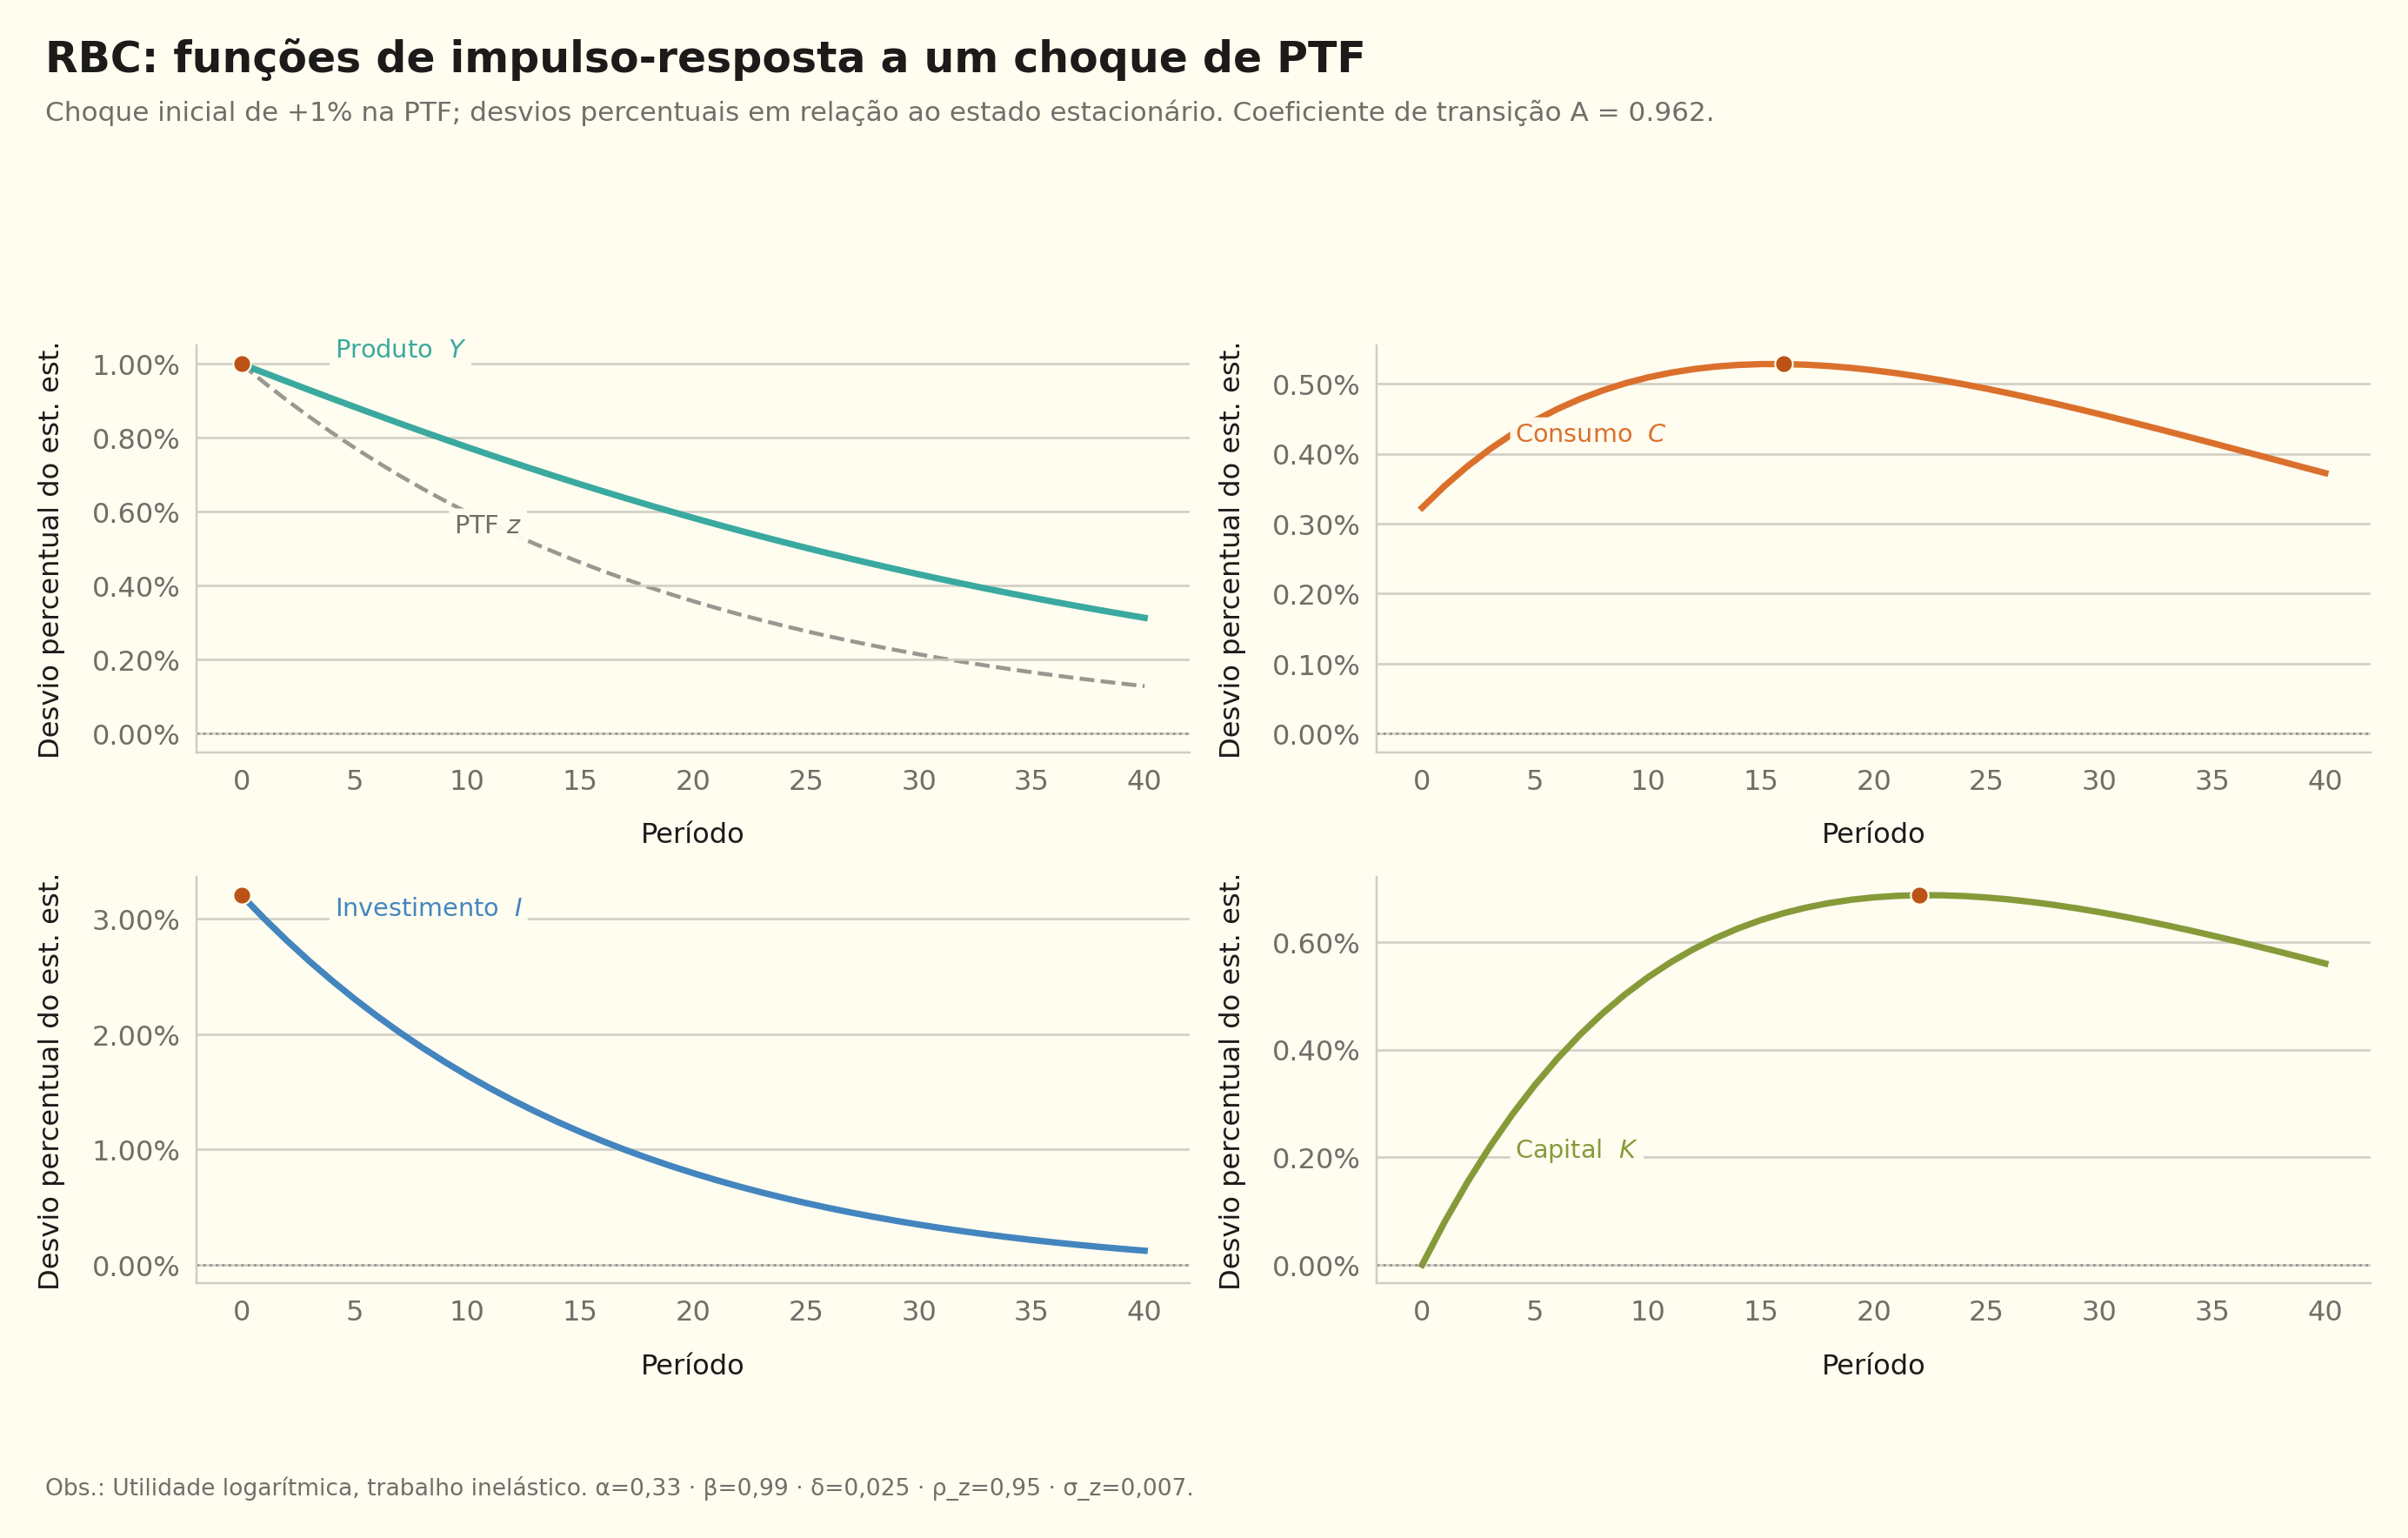
\includegraphics[width=0.85\textwidth]{rbc_irf.png}
\caption{FRI do modelo RBC: $\hat{I}_0 > \hat{Y}_0 > \hat{C}_0$ --- os três canais.}
\end{figure}

\begin{figure}[H]
\centering
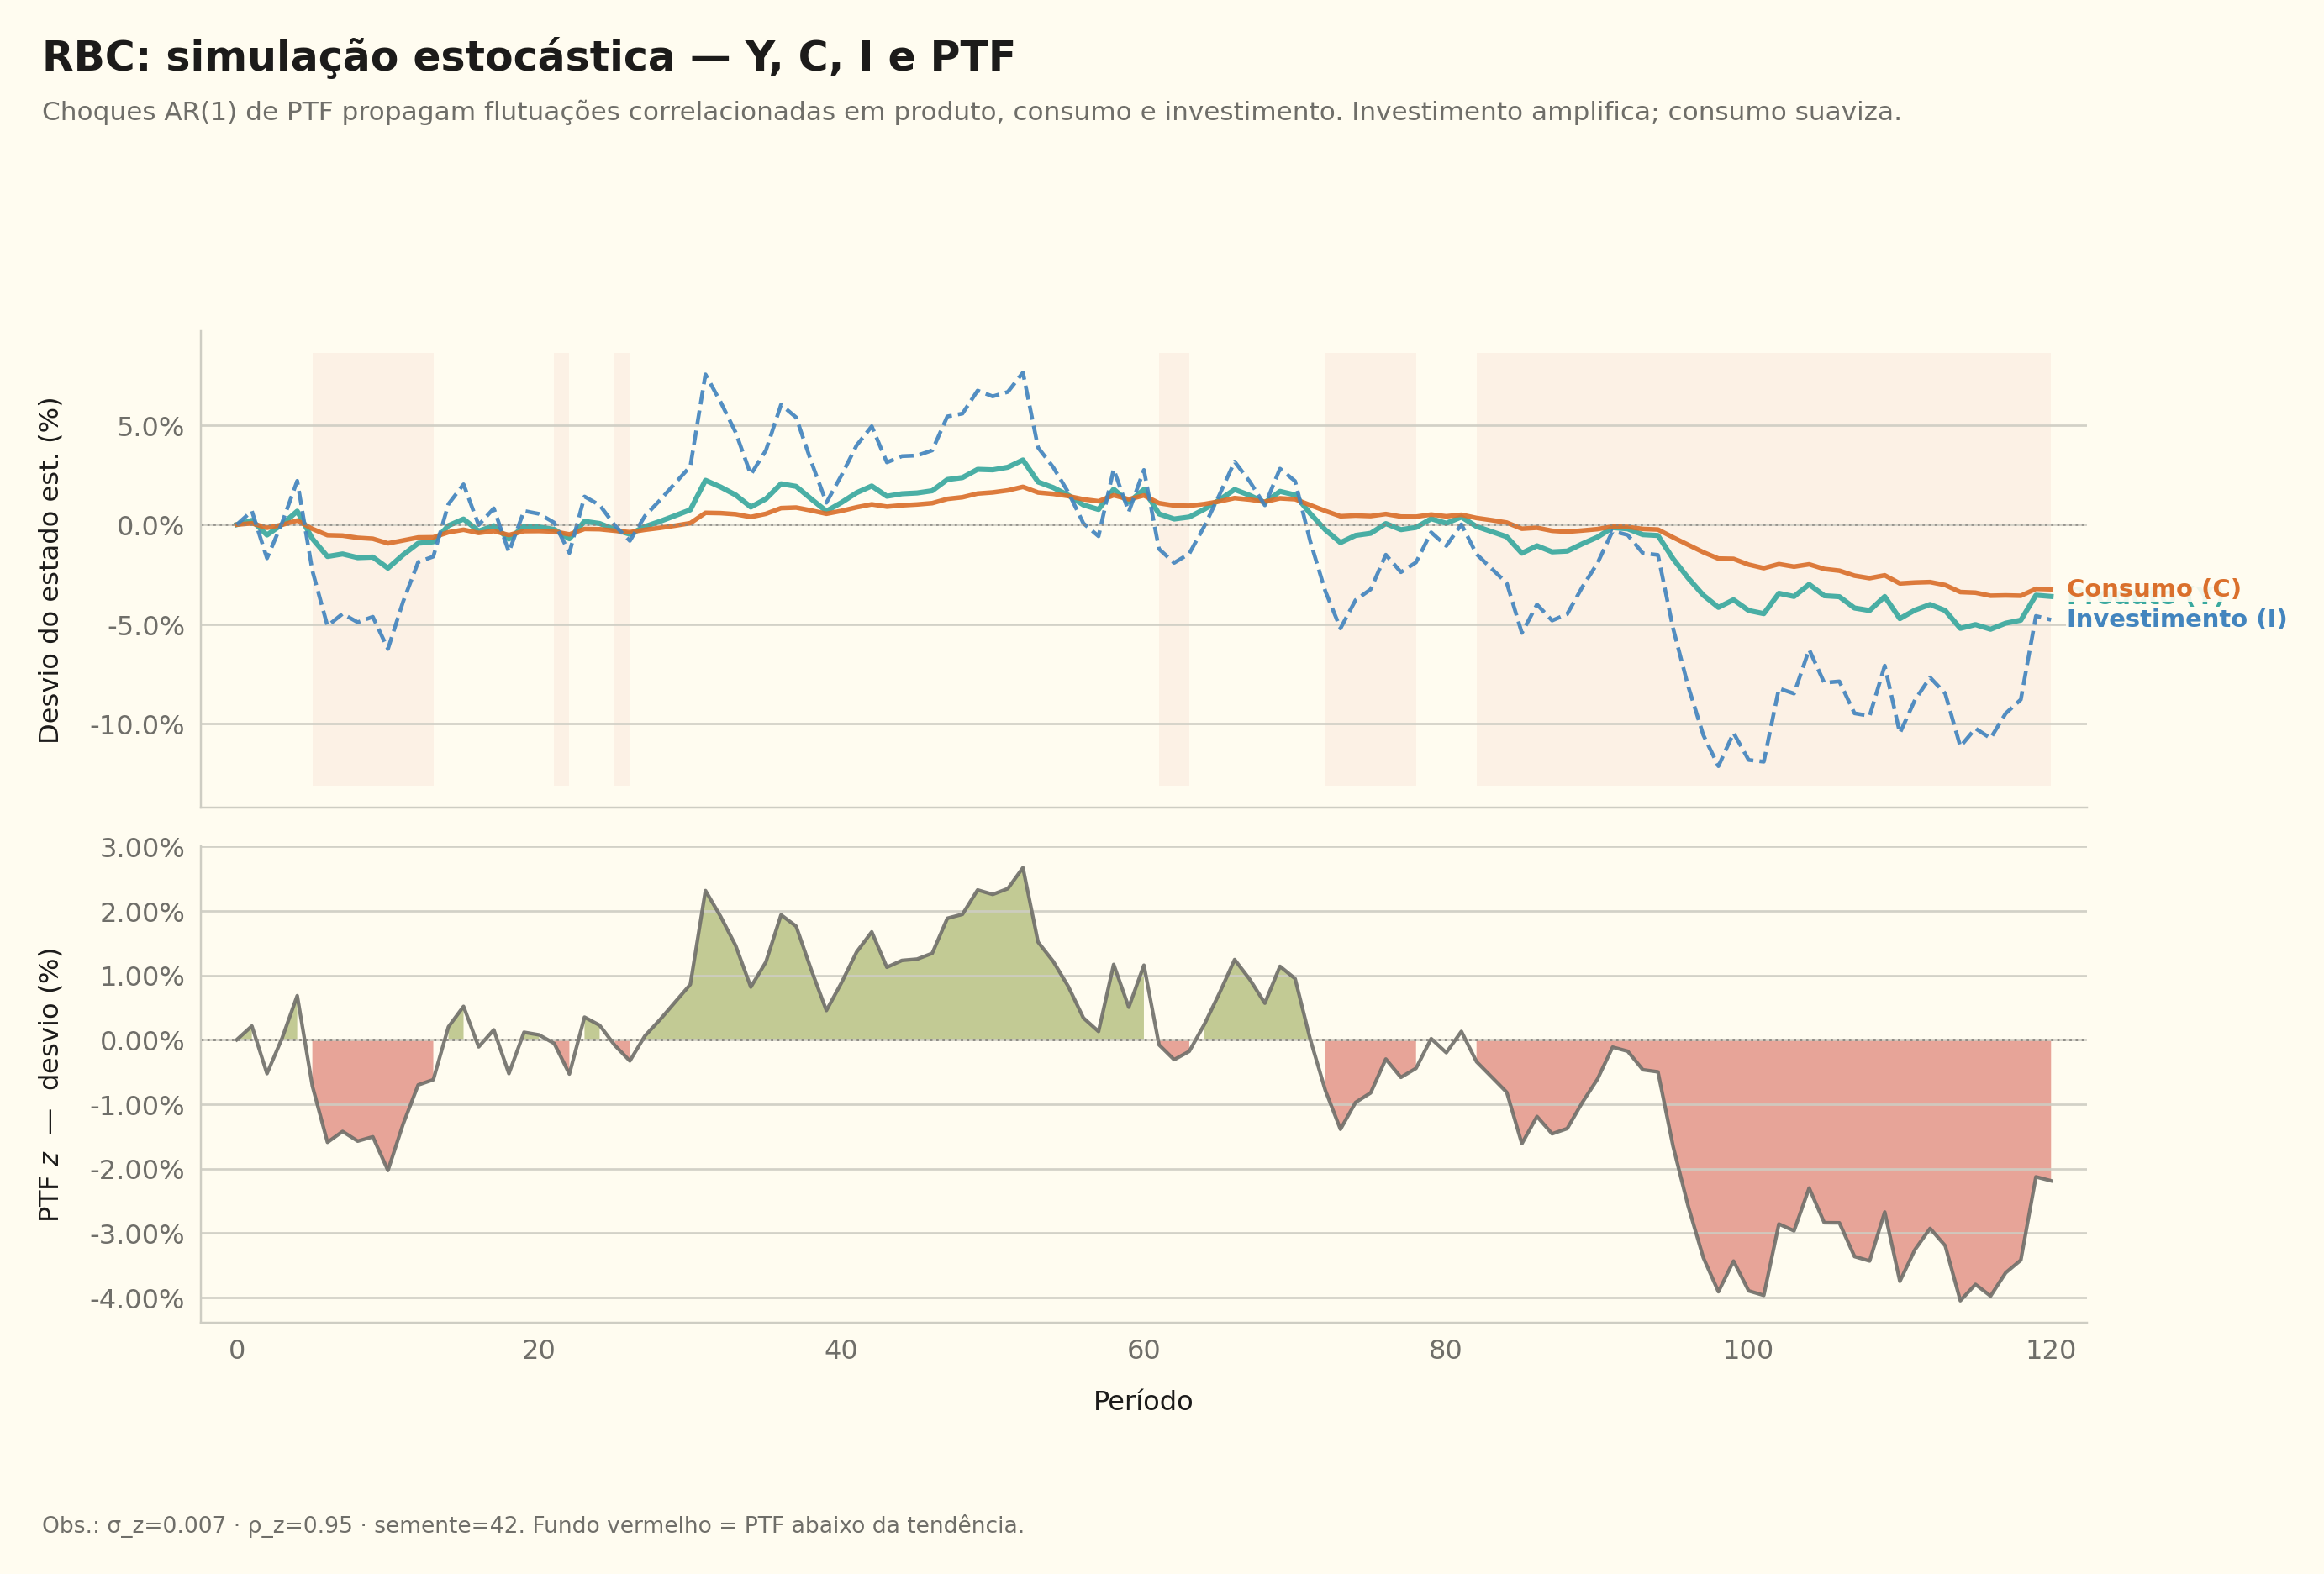
\includegraphics[width=0.85\textwidth]{rbc_simulation.png}
\caption{Simulação estocástica: séries $Y$, $C$, $I$ e $z_t$. Notar $\sigma_I > \sigma_Y > \sigma_C$.}
\end{figure}

\begin{figure}[H]
\centering
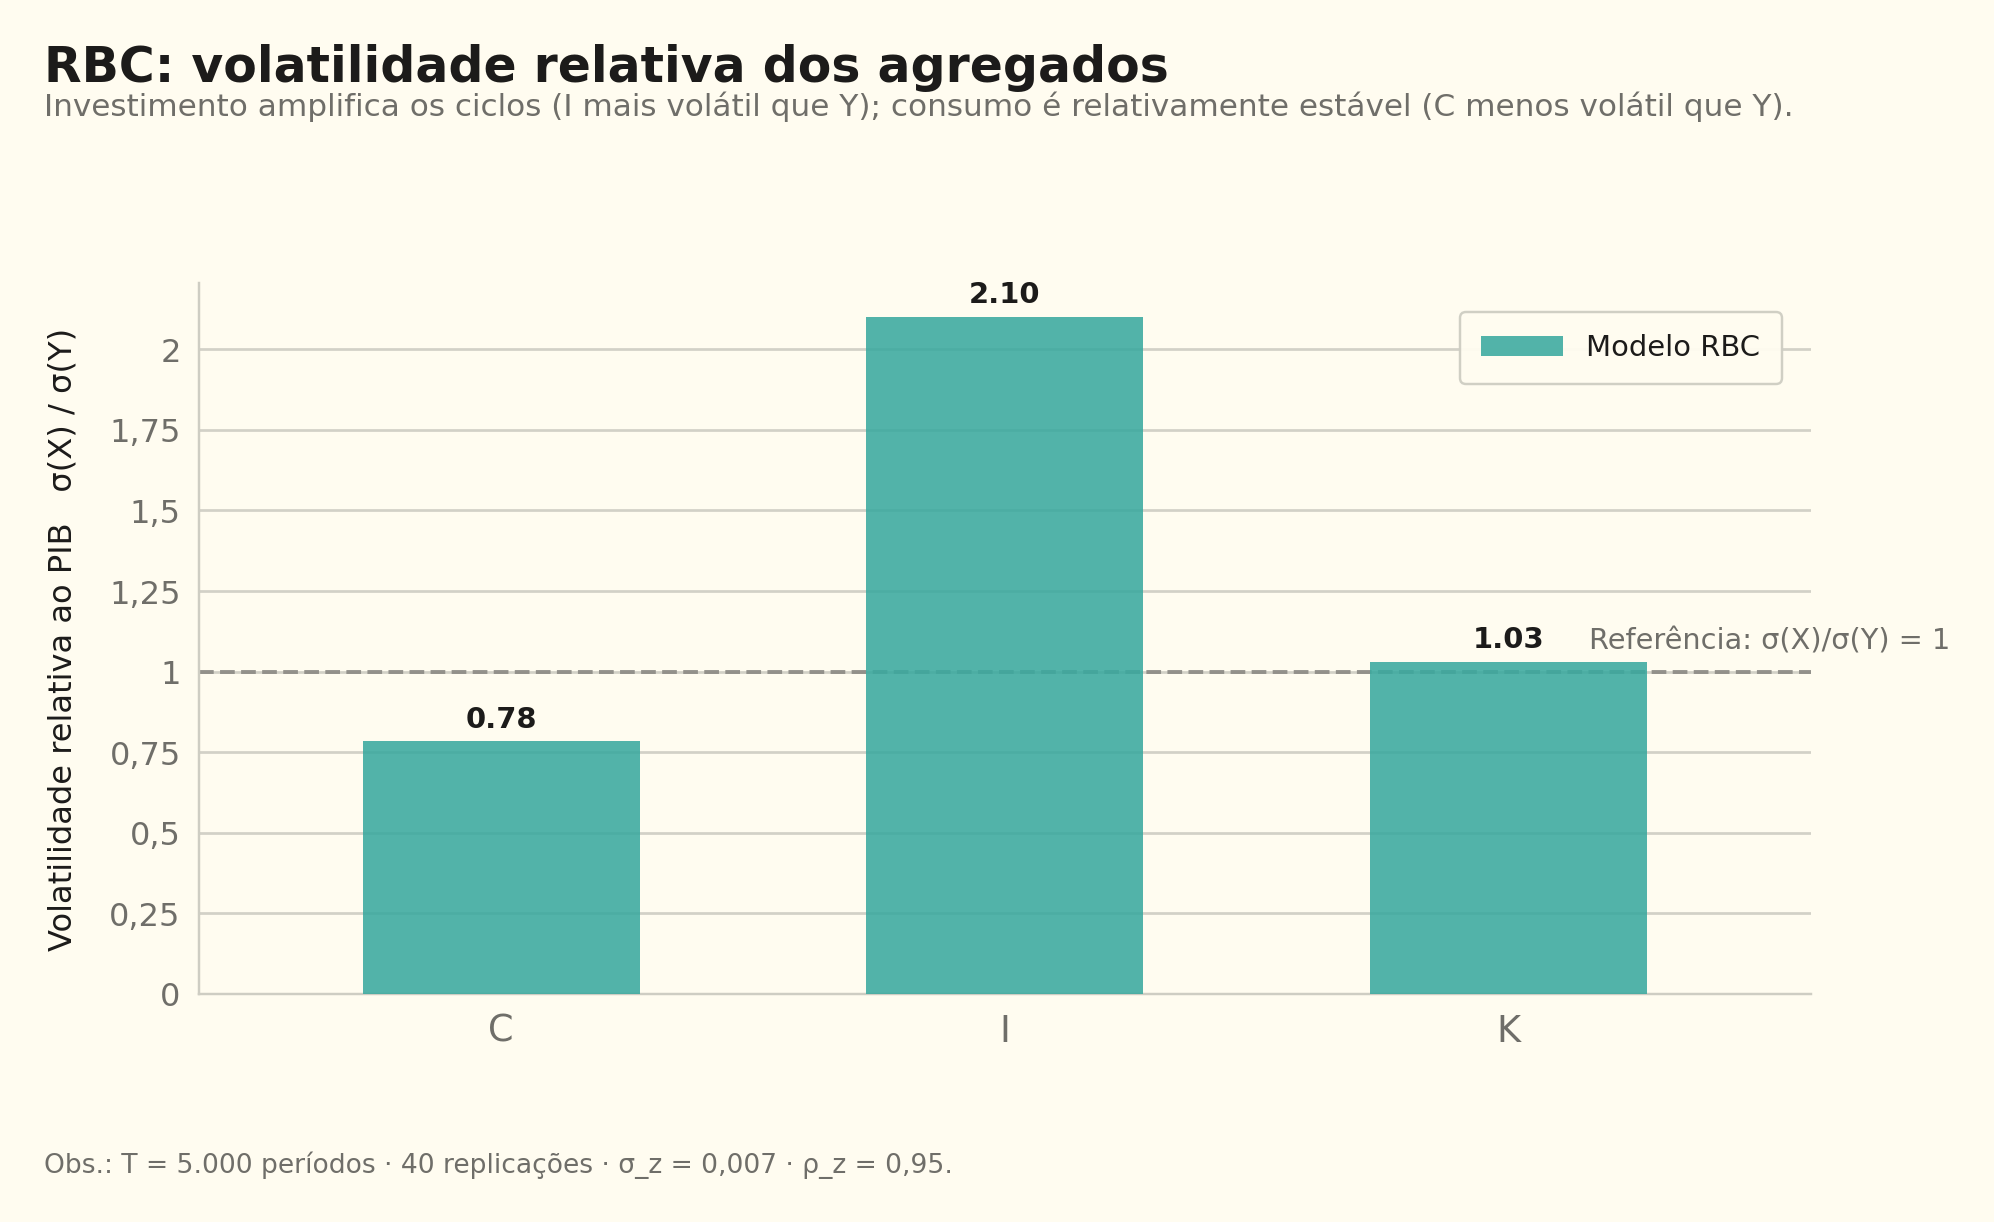
\includegraphics[width=0.85\textwidth]{rbc_moments.png}
\caption{Momentos do modelo RBC: $\sigma(I)/\sigma(Y) > 1 > \sigma(C)/\sigma(Y)$.}
\end{figure}

% ==========================================================================
%  Apêndice — Questões-tipo P1
% ==========================================================================

\newpage
\appendix
\renewcommand{\thesection}{Q-tipo}
\section*{\color{cyanrbc} Apêndice --- Questões-tipo P1 (estilo P1 2024)}
\addcontentsline{toc}{section}{Apêndice --- Questões-tipo P1}

As questões abaixo reproduzem o formato exato da P1 2024 (múltipla escolha,
4 alternativas, uma correta). Resolva antes de verificar a resposta.

\bigskip

% ------------------------------------------------------------------
\subsection*{Q-tipo 1 --- RCK: Equação de Keynes-Ramsey}

Com base na equação de Keynes-Ramsey $\dot{c}/c = (r-\rho)/\theta$, identifique
a \textbf{alternativa verdadeira}:

\begin{enumerate}[label=\textbf{\alph*)}, leftmargin=2em, itemsep=4pt]
  \item A elasticidade de substituição intertemporal é igual a $\theta$.
  \item A taxa de desconto $\rho$ afeta \textbf{negativamente} a taxa de crescimento
    do consumo.
  \item A condição de crescimento equilibrado exige $\rho - n + (1-\theta)g > 0$.
  \item Quanto menor $\theta$, menor a sensibilidade do consumo a mudanças em $r$.
\end{enumerate}

\begin{resultbox}[title={Resposta Q-tipo 1: alternativa b)}]
\textbf{Correta: b)}

\textit{Justificativa:} $\dot{c}/c = (r-\rho)/\theta$ mostra que $\rho$ aparece
com sinal negativo: $\partial(\dot{c}/c)/\partial\rho = -1/\theta < 0$.
Impaciência maior ($\rho\uparrow$) reduz o incentivo a acumular.

\textit{Por que as outras estão erradas:}
\begin{itemize}[leftmargin=1.5em, topsep=2pt, itemsep=2pt]
  \item a) Falso: a EIS é $1/\theta$, não $\theta$.
  \item c) Falso: a condição correta é $\rho - n - (1-\theta)g > 0$ (sinal $-$, não $+$).
  \item d) Falso: $1/\theta$ mede sensibilidade; $\theta$ \textit{menor} implica
    $1/\theta$ \textit{maior} $\Rightarrow$ \textit{maior} sensibilidade.
\end{itemize}
\end{resultbox}

\bigskip

% ------------------------------------------------------------------
\subsection*{Q-tipo 2 --- RBC: Substituição intertemporal de trabalho}

No modelo RBC com lazer, um aumento da taxa real de juros:

\begin{enumerate}[label=\textbf{\alph*)}, leftmargin=2em, itemsep=4pt]
  \item Aumenta o lazer corrente via efeito riqueza.
  \item Reduz a oferta de trabalho presente via substituição intertemporal.
  \item Eleva a oferta de trabalho hoje relativamente ao futuro.
  \item Não altera a oferta de trabalho por ser um choque nominal.
\end{enumerate}

\begin{resultbox}[title={Resposta Q-tipo 2: alternativa c)}]
\textbf{Correta: c)}

\textit{Justificativa:} Da fórmula $\dfrac{1-l_1}{1-l_2} = \beta(1+r)\dfrac{w_2}{w_1}$,
um aumento em $r$ eleva o lado direito $\Rightarrow$ $N_1/N_2\uparrow$: trabalha-se
mais hoje relativamente ao futuro (substituição intertemporal de lazer).

\textit{Por que as outras estão erradas:}
\begin{itemize}[leftmargin=1.5em, topsep=2pt, itemsep=2pt]
  \item a) Falso: $r\uparrow$ deprime $C_t$ (Euler), logo $l_t^*=bC_t/w_t$ cai.
  \item b) Falso: $r\uparrow$ \textit{eleva} (não reduz) a oferta de trabalho presente.
  \item d) Falso: $r$ é taxa real; afeta diretamente o trade-off intertemporal.
\end{itemize}
\end{resultbox}

\bigskip

% ------------------------------------------------------------------
\subsection*{Q-tipo 3 --- RBC: Estabilidade do capital}

No estado estacionário do modelo RBC, qual a condição para estabilidade do capital?

\begin{enumerate}[label=\textbf{\alph*)}, leftmargin=2em, itemsep=4pt]
  \item $I^* > \delta K^*$
  \item $I^* = \delta K^*$
  \item $\beta(r^* - 1 + \delta) = 1$
  \item $A = 1$
\end{enumerate}

\begin{resultbox}[title={Resposta Q-tipo 3: alternativa b)}]
\textbf{Correta: b)}

\textit{Justificativa:} No EE, $K_{t+1}=K_t$ implica $I_t = \delta K_t$.
O investimento líquido é zero: toda a poupança repõe a depreciação.

\textit{Por que as outras estão erradas:}
\begin{itemize}[leftmargin=1.5em, topsep=2pt, itemsep=2pt]
  \item a) $I^*>\delta K^*$ significaria capital crescendo, não estacionário.
  \item c) A Euler correta é $\beta(r^*+1-\delta)=1$, não $\beta(r^*-1+\delta)=1$
    (sinal trocado).
  \item d) $A=1$ seria raiz unitária --- sem convergência, sistema instável.
\end{itemize}
\end{resultbox}

\bigskip

% ------------------------------------------------------------------
\subsection*{Q-tipo 4 --- RCK: Diagrama de fases}

No diagrama de fases do modelo RCK, uma economia posicionada à \textbf{direita} do
locus $\dot{c}=0$ e \textbf{abaixo} do locus $\dot{k}=0$ apresenta:

\begin{enumerate}[label=\textbf{\alph*)}, leftmargin=2em, itemsep=4pt]
  \item $\dot{c}<0$ e $\dot{k}<0$
  \item $\dot{c}<0$ e $\dot{k}>0$
  \item $\dot{c}>0$ e $\dot{k}>0$
  \item $\dot{c}>0$ e $\dot{k}<0$
\end{enumerate}

\begin{resultbox}[title={Resposta Q-tipo 4: alternativa b)}]
\textbf{Correta: b)}

\textit{Justificativa:}
\begin{itemize}[leftmargin=1.5em, topsep=2pt, itemsep=2pt]
  \item \textbf{À direita de $\dot{c}=0$}: $k > \kstar \Rightarrow f'(k) < \rho+\theta g$
    $\Rightarrow \dot{c}<0$ (consumo cai).
  \item \textbf{Abaixo de $\dot{k}=0$}: dado $k$, $c$ é baixo demais para zerar acumulação
    $\Rightarrow$ poupança supera depreciação $\Rightarrow \dot{k}>0$ (capital acumula).
\end{itemize}
Portanto: $\dot{c}<0$ e $\dot{k}>0$ --- setas para sudeste. Esta região converge
à trajetória de sela (equilíbrio estável).

\textit{Por que as outras estão erradas:}
\begin{itemize}[leftmargin=1.5em, topsep=2pt, itemsep=2pt]
  \item a) Errado o sinal de $\dot{k}$ (abaixo $\Rightarrow \dot{k}>0$).
  \item c), d) Errado o sinal de $\dot{c}$ (direita $\Rightarrow \dot{c}<0$).
\end{itemize}
\end{resultbox}

\bigskip

% ==========================================================================
%  Apêndice B — Log-linearização e Calibração
% ==========================================================================

\section*{\color{cyanrbc} Apêndice B --- Log-linearização e Calibração}
\addcontentsline{toc}{section}{Apêndice B --- Log-linearização e Calibração}

\subsection*{Log-linearização do modelo RBC}

Supõe-se política de consumo linear nos estados:
$\chat_t = a_k\khat_t + a_z\zhat_t$.

\textbf{Capital:}
\[
\khat_{t+1} = \gamma_k\khat_t + \gamma_z\zhat_t - \gamma_c\chat_t,
\]
onde $\gamma_k=(1-\delta)+\alpha\,iy$, $\gamma_z=iy$, $\gamma_c=cy$,
com $iy=I^*/Y^*$ e $cy=C^*/Y^*$.

\textbf{Euler:}
\[
\chat_t = \chat_{t+1} - \beta\rstar[\zhat_{t+1}+(\alpha-1)\khat_{t+1}].
\]

\textbf{Quadrática para $a_k$:}
\[
-\gamma_c\,a_k^2 + (\gamma_k - 1 - m\gamma_c)\,a_k + m\gamma_k = 0,
\quad m = \beta\rstar(1-\alpha).
\]
Raiz estável: $a_k\approx 0.590$, $A\approx 0.962$.

\begin{table}[H]
\centering
\caption{Parâmetros de calibração (RCK e RBC).}
\begin{tabular}{llll}
\toprule
\multicolumn{2}{c}{Modelo RCK} & \multicolumn{2}{c}{Modelo RBC} \\
\cmidrule(r){1-2}\cmidrule(l){3-4}
Parâmetro & Valor & Parâmetro & Valor \\
\midrule
$\alpha$ & 0.33 & $\alpha$ & 0.33 \\
$\rho$ (desconto) & 0.02 & $\beta$ & 0.99 \\
$n$ (crescimento pop.) & 0.01 & $\delta$ & 0.025 \\
$g$ (progresso técnico) & 0.02 & $\rho_z$ & 0.95 \\
$\delta$ (deprec.) & 0.05 & $\sigma_z$ & 0.007 \\
$\theta$ (CRRA) & 1.5 & $b$ (lazer) & $\approx 1.55$ \\
\bottomrule
\end{tabular}
\end{table}

\bigskip
\hrule
\vspace{1em}
{\footnotesize
\textbf{Código-fonte:} \url{https://github.com/fcarva/macro} ---
pastas \texttt{ch02\_rck\_diamond/} e \texttt{ch05\_rbc/}.
Requer Python $\geq$ 3.11, \texttt{numpy}, \texttt{scipy}, \texttt{matplotlib}.
}

\end{document}
